% !TeX root = ../tfg.tex
% !TeX encoding = utf8

\chapter{Análisis teórico del Deep Double Descent}\label{ch:analisis-teorico-ddd}

En este capítulo, nos vamos a encargar de abordar, de manera teórica, el doble descenso profundo. En primer lugar, lo definiremos con la mayor precisión posible, ofreciendo una intuición clara a partir de un problema de regresión. A continuación, se presentarán los principales desarrollos presentes en la literatura científica, así como algunos avances recientes en el tema. Para concluir el capítulo, se abordará la teoría de la aproximación no lineal, ya que, a priori, presenta ciertas analogías con este fenómeno.\newline

\section{Planteamiento teórico}\label{sec:planteamiento-teorico}

Siguiendo los resultados expuestos en la Sección~\ref{sec:subsec-underfitting-y-overfitting}, la sabiduría clásica adopta una visión en la cual sostiene que los modelos más grandes tienden a ser peores, ya que su capacidad de generalización empeora. En la práctica moderna, especialmente ahora en la era del \textit{deep learning}, es cada vez más común el uso de modelos de gran tamaño con suficientes parámetros para reducir el error de entrenamiento casi a cero. A pesar de ajustarse casi perfectamente a los datos, estos modelos logran generalizar sorprendentemente bien e incluso superar en rendimiento a modelos más simples.\newline

De esta manera, se ha comprobado que, más allá de cierto umbral, el aumento de la capacidad de los modelos resulta beneficioso, ya que no conduce al sobreajuste y, en realidad, disminuye nuevamente el error de generalización. A esta nueva zona de funcionamiento de los modelos la denotaremos como \emph{régimen moderno} o zona sobreparametrizada, mientras que la región previa al umbral, en la que se produce la tradicional curva con forma de ``U'', la denominaremos como \textit{régimen clásico} o zona infraparametrizada.\newline

De cara a formalizar el fenómeno del doble descenso profundo y unificar la sabiduría clásica con la práctica moderna, introducimos una nueva medida de capacidad del modelo, propuesta por Nakkiran et al.\ en~\cite{Nakkiran2019}.

\begin{definicion}[Complejidad efectiva del modelo]
    La complejidad efectiva del modelo (EMC, por sus siglas en inglés) de un algoritmo de aprendizaje $\mathcal{A}$, con respecto a la distribución de probabilidad conjunta $P[X, Y]$ de los datos del conjunto de entrenamiento $\mathcal{D}$, es el máximo número de ejemplos de entrenamiento $n$ en el que $\mathcal{A}$ obtiene, de media, un error de entrenamiento muy próximo a cero. Es decir, dado $\epsilon > 0$:

    \[
        EMC_{P, \epsilon}(\mathcal{A}) = \max\{ n \in \mathbb{N} \; | \; \mathbb{E}[L(g)] \leq \epsilon \}
    \]  

    donde $L(g)$ hace referencia a la función de pérdida de la función candidata $g \in \mathcal{H}$.\newline
\end{definicion}

Una vez definida la noción de complejidad efectiva del modelo, se expone uno de los resultados principales de este trabajo.

\begin{hipotesis}\label{hipotesis-general-double-descent}
    Para cualquier distribución de datos $P[X, Y]$, algoritmo de aprendizaje basado en redes neuronales $\mathcal{A}$ (véase Subsección~\ref{subsubsec:aprendizaje-red-neuronal}) y un pequeño $\epsilon > 0$, si consideramos la tarea de predecir etiquetas basadas en $n$ muestras aleatorias e independientes de $P[X, Y]$, entonces:

    \begin{itemize}
        \item \textbf{Región infraparametrizada.} Si $EMC_{P, \epsilon}(\mathcal{A})$ es suficientemente menor que $n$, entonces cualquier perturbación de $\mathcal{A}$ que aumente su complejidad efectiva, disminuirá su error de generalización.
        \item \textbf{Región crítica.} Si $EMC_{P, \epsilon}(\mathcal{A}) \approx n$, entonces cualquier perturbación de $\mathcal{A}$ que aumente su complejidad efectiva puede aumentar o disminuir su error de generalización.
        \item \textbf{Región sobreparametrizada.} Si $EMC_{P, \epsilon}(\mathcal{A})$ es suficientemente mayor que $n$, entonces cualquier perturbación de $\mathcal{A}$ que aumente su complejidad efectiva, disminuirá su error de generalización.\newline
    \end{itemize}
\end{hipotesis}

Esta hipótesis es informal en varios sentidos. En primer lugar, no disponemos de una forma precisa de elegir el parámetro $\epsilon$, ni de una especificación formal para ``suficientemente pequeño'' y ``suficientemente grande''. La hipótesis sugiere que hay un intervalo crítico alrededor del umbral de interpolación $(EMC_{P, \epsilon}(\mathcal{A}) = n)$ de manera que, tanto por debajo como por encima de dicho intervalo, el aumento de la complejidad beneficia el rendimiento del modelo, mientras que en el interior de este intervalo el comportamiento es incierto, pudiendo mejorar o empeorar. Además, la amplitud de dicho intervalo depende tanto de la distribución de los datos del conjunto de entrenamiento $\mathcal{D}$ como del algoritmo de aprendizaje $\mathcal{A}$ utilizado.\newline

\begin{figure}[h]
    \centering
    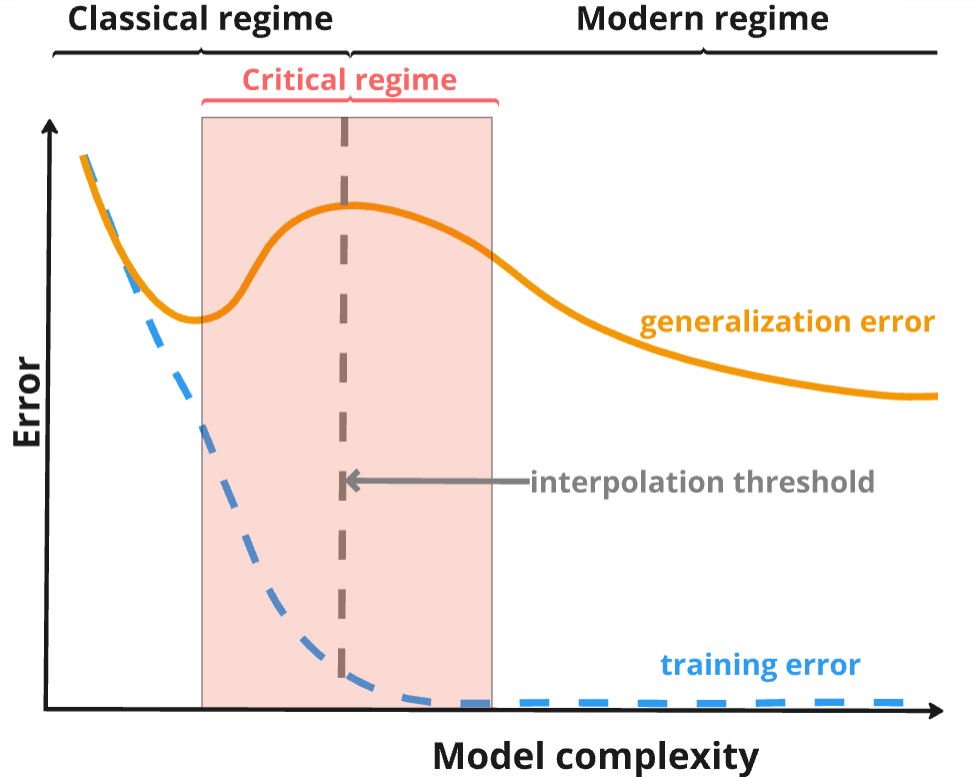
\includegraphics[width=0.65\linewidth]{img/planteamiento-teorico-dd.png}
    \caption[Ejemplo de doble descenso con las distintas zonas de parametrización.]{Ejemplo de doble descenso con las distintas zonas de parametrización. Se puede observar la tradicional forma de ``U'' en la zona clásica, seguida de la zona crítica, donde el error de generalización es incierto, ya que puede aumentar o disminuir, y, finalmente, la zona moderna, donde el error de generalización es incluso menor que el obtenido en la zona clásica.}\label{fig:planteamiento-teorico-dd.png}
\end{figure}

Por otra parte, la Hipótesis~\ref{hipotesis-general-double-descent} nos ayuda a unificar la sabiduría clásica con los resultados modernos en una curva de aprendizaje que abarca ambos mundos. Hasta el umbral de interpolación, la curva sigue la tradicional forma de ``U'', cuyo mínimo se alcanza en el \textit{sweet spot} (véase Figura~\ref{fig:biasvarianceunderoverfitting}) mientras que, aumentando la capacidad del modelo hasta alcanzar un error de entrenamiento muy próximo a cero, y tras superar la zona crítica donde se encuentra el umbral de interpolación, nos indica que el error de generalización comienza nuevamente a disminuir, pudiendo lograr un error menor que el obtenido en el \textit{sweet spot}.\newline

Este comportamiento, en el que la curva del error de generalización exhibe dos descensos, puede apreciarse en la Figura~\ref{fig:planteamiento-teorico-dd.png} y lo denotaremos como \textbf{doble descenso profundo}, o simplemente \textbf{doble descenso}. En este contexto, el adjetivo \textit{profundo} hace referencia al uso de redes neuronales profundas como modelo base.\newline

Aun habiendo unificado ambos puntos de vista, la descomposición del error en términos de sesgo y varianza, tal como se mencionó en la Sección~\ref{sec:capitulo-bias-variance-tradeoff}, sugiere que uno de estos dos componentes, tras alcanzar el valor máximo de error, comienza nuevamente a disminuir. La Figura~\ref{fig:bias-variance-peak} ilustra los tres comportamientos distintos que pueden surgir como resultado de dicha descomposición. Para nuestro análisis, resulta razonable suponer que es la varianza la que disminuye tras alcanzar el punto máximo del error, ya que sabemos que este término predomina a partir del \textit{sweet spot}, dando lugar a una curva unimodal.\newline

\begin{figure}[h]
    \centering
    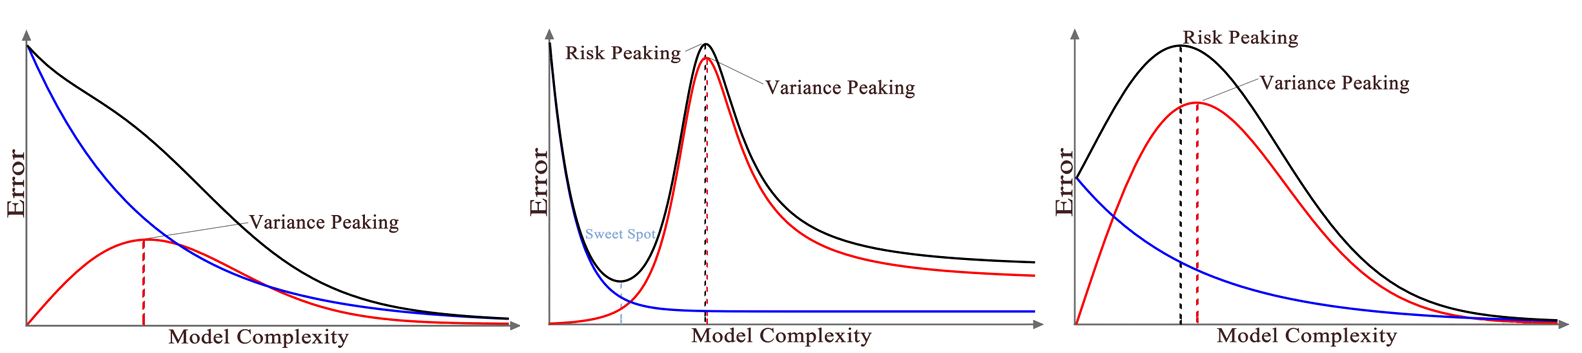
\includegraphics[width=0.8\linewidth]{img/bias-variance-peak.png}
    \caption[Curvas típicas del error en función del sesgo y la varianza~\cite{Yang2020}.]{Curvas típicas del error (línea negra) en función del sesgo (línea azul) y la varianza (línea roja)~\cite{Yang2020}. A la izquierda, el término de sesgo domina completamente, lo que da lugar a un error decreciente. En la región central, el sesgo y la varianza predominan en zonas distintas, produciéndose así el doble descenso. Finalmente, a la derecha, el término de varianza se vuelve dominante, generando una curva con forma de campana en la que el error inicialmente aumenta.}\label{fig:bias-variance-peak}
\end{figure}

De este modo, a medida que aumenta la capacidad del modelo, esto implica que, a pesar de disponer de un conjunto de hipótesis más amplio, el modelo se está concentrando en un subconjunto específico de dichas hipótesis, lo que reduce el error asociado a la varianza.\newline

A modo de resumen, estamos separando las distintas zonas de funcionamiento de un modelo en función, en cierta medida, de su conjunto de hipótesis $\mathcal{H}$. En la zona clásica, por lo general, no existe ninguna hipótesis que minimice completamente el riesgo real, es decir, no existe $g \in \mathcal{H}$ tal que $L(g) = 0$. Por el contrario, en la zona moderna, conforme aumenta la capacidad del modelo, aparece un conjunto cada vez más amplio $S \subset \mathcal{H}$ que interpola a la perfección los datos de entrenamiento. Este conjunto se define como:  

\[
    S = \{ g \in \mathcal{H} \mid L(g) = 0 \}.
\]

En consecuencia, el verdadero problema radica en comprender por qué el algoritmo de aprendizaje $\mathcal{A}$, en la zona sobreparametrizada, tiende a seleccionar ``buenas'' soluciones dentro del conjunto $S$, es decir, aquellas que logran una buena generalización. Es importante destacar que esta cuestión no se puede responder únicamente a partir de los datos del conjunto de entrenamiento $\mathcal{D}$, ya que cualquier hipótesis de $S$ se ajusta perfectamente a esos datos. Por tanto, la clave para comprender el fenómeno vendrá dada por el sesgo inductivo que presentan algunos de los algoritmos de optimización más comunes, los cuales favorecen ciertas soluciones dentro de $S$.\newline

\subsection{Análisis intuitivo en un problema de mínimos cuadrados}\label{subsec:analisis-intuitivo-minimos-cuadrados}

De cara a ofrecer una primera intuición sencilla sobre la ocurrencia del doble descenso, consideramos un problema de regresión lineal (basado en~\cite{Schaeffer2023}) que resolveremos utilizando el método de mínimos cuadradados ordinarios (OLS), cuya solución de norma mínima viene dada por la pseudoinversa, como vimos en la Sección~\ref{sec:svd-pseudoinversa}. Además, para comprender dónde y cómo se produce este suceso, estudiaremos las dos zonas de parametrización del modelo de regresión lineal, analizando los diferentes errores que se producen en cada una de ellas.\newline

Supongamos que nos enfrentamos ante un problema de regresión lineal en el que disponemos de $N$ ejemplos, donde cada ejemplo está formado por los respectivos datos de entrada y su correspondiente etiqueta. Sea $D$ la dimensión de los puntos de entrenamiento y $P$ el número de parámetros a ajustar para realizar la regresión lineal. De esta manera, nuestro conjunto de entrenamiento $\mathcal{D}$ está formado por $N$ pares de la forma $(x,y)$, donde $x \in \mathbb{R}^{D}$ representa un punto en el plano $D$-dimensional e $y \in \mathbb{R}$ la variable objetivo.\newline

Para resolver el problema de regresión lineal, debemos abordar el clásico problema de minimización de mínimos cuadrados, formulado como sigue

\begin{equation}\label{eq:minimos-cuadrados1}
    \arg\min_{w} \frac{1}{N}\sum_{n=1}^{N}\| x_n \cdot w - y_n \|^{2} = \arg\min_{w}\| Xw - Y \|^{2}
\end{equation}

donde cada par $(x, y)$ representa un ejemplo de entrenamiento y $w$ indica el vector de pesos o parámetros que queremos aprender de cara a realizar la aproximación. Además, $X \in \mathcal{M}_{N \times D}(\mathbb{R})$ y $Y\in \mathcal{M}_{N \times 1}(\mathbb{R})$ representan, respectivamente, los puntos de entrenamiento y su correspondiente salida en forma matricial.\newline

En la zona infraparametrizada, es decir, cuando el número de ejemplos de entrenamiento es mayor que el número de parámetros a ajustar $(P < N)$, la solución al problema de minimización~\eqref{eq:minimos-cuadrados1}, ofrecida por la pseudoinversa de $X$, viene dada por ${(X^{T}X)}^{-1}X^{T}$. De este modo, el vector de pesos $w$ puede ser expresado como:

\begin{equation}
    w_{under} = {(X^{T}X)}^{-1}X^{T}Y.
\end{equation}\newline

Por otra parte, en la zona sobreparametrizada, es decir, cuando el número de parámetros es mayor que el número de ejemplos de entrenamiento $(N < P)$, no se puede resolver el problema de minimización~\eqref{eq:minimos-cuadrados1} de manera convencional, dado que estaría mal planteado, debido al hecho de que existirían múltiples soluciones, ya que habría menos restricciones que parámetros. Por tanto, debemos de seleccionar un problema de optimización distinto, que también se encuentre sujeto a las restricciones impuestas por los ejemplos de entrenamiento. En este contexto, elegimos el problema más simple que se podría imaginar, dado por:

\begin{equation}\label{eq:minimos-cuadrados2}
    \arg\min_{w}\| w \|^{2}, \quad \text{sujeto a} \; \forall n \in \{1, \ldots, N\} \quad x_n \cdot w = y_n.
\end{equation}\newline

El problema de optimización~\eqref{eq:minimos-cuadrados2} busca el vector de parámetros con menor norma que satisface $x_n \cdot w = y_n$ para todos los ejemplos de entrenamiento. La solución a este problema de optimización también se obtiene mediante la pseudoinversa, pero en este caso, la pseudoinversa se calcula conociendo que la matriz $X$ tiene rango completo en esta región y cuenta con filas linealmente independientes. Así, la pseudoinversa viene dada por $X^{T}{(XX^{T})}^{-1}$ (véase~\ref{sec:svd-pseudoinversa}). De esta forma, el vector de pesos $w$ puede ser expresado como:

\begin{equation}
    w_{over} = X^{T}{(XX^{T})}^{-1}Y.
\end{equation}\newline

Por tanto, una vez que se ha obtenido el vector de pesos, el modelo realizará las siguientes predicciones para un determinado punto de prueba $x_{\text{test}}$, dependiendo de la zona de parametrización en la que se encuentre:

\begin{equation}
    y_{test, under} = x_{\text{test}} \cdot w_{\text{under}} = x_{\text{test}} \cdot {(X^{T}X)}^{-1}X^{T}Y.
\end{equation}

\begin{equation}
    y_{test, over} = x_{\text{test}} \cdot w_{\text{over}} = x_{\text{test}} \cdot X^{T}{(XX^{T})}^{-1}Y.
\end{equation}\newline

No obstante y llegados a este punto, las diferencias al predecir un punto de prueba en ambas zonas de parametrización no parecen ser del todo claras. Para identificar estas diferencias con mayor precisión, reescribiremos nuestras predicciones de la siguiente forma:

\[
    y_n = x_n \cdot w^{*} + e_n
\]

donde $w^{*} \in \mathbb{R}^{P} = \mathbb{R}^{D}$ representa el vector de parámetros ideal que realmente minimiza el error cuadrático medio y $e_n$ representa un término de error adicional presente en la propia naturaleza de los datos, es decir, un residuo que el modelo no puede capturar. Equivalentemente, en forma matricial, podemos escribir:

\[
    Y = X \cdot w^{*} + E \quad \text{con } E \in \mathbb{R}^{N \times 1}.
\]\newline

Usando esta notación, podemos reformular las predicciones que realiza el modelo. De esta manera, para el caso de la zona infraparametrizada nos queda:

\begin{align}
    y_{test, under} &= x_{test} \cdot {(X^T X)}^{-1} X^T Y \\
    &= x_{test} \cdot {(X^T X)}^{-1} X^T (X w^{*} + E) \\
    &= x_{test} \cdot {(X^T X)}^{-1} X^T X w^{*} + x_{test} \cdot {(X^T X)}^{-1} X^T E \\
    &= \underbrace{x_{test} \cdot w^{*}}_{\overset{def}{=} y^*_{test}} + x_{test} \cdot {(X^T X)}^{-1} X^T E
\end{align}

\begin{equation}
    y_{test, under} - y^{*}_{test} = x_{test} \cdot {(X^T X)}^{-1} X^T E.
\end{equation}\newline

Por otra parte, para el caso de la zona sobreparametrizada, los cálculos serían los siguientes:

\begin{align}
    y_{test, over} &= x_{test} \cdot X^{T}{(XX^{T})}^{-1}Y \\
    &= x_{test} \cdot X^{T}{(XX^{T})}^{-1}(X w^{*} + E) \\
    &= x_{test} \cdot X^{T}{(XX^{T})}^{-1}X w^{*} + x_{test}X^{T}{(XX^{T})}^{-1}E \\
    y_{test, over} - \underbrace{x_{test} \cdot w^{*}}_{\overset{def}{=} y^*_{test}} &= x_{test} \cdot X^{T}{(XX^{T})}^{-1}X w^{*} - x_{test} \cdot I_{D} w^{*} + x_{test} \cdot {(X^{T}X)}^{-1}X^{T}E
\end{align}

\begin{equation}
    y_{test, over} - y^{*}_{test} = x_{test} \cdot (X^{T}{(XX^{T})}^{-1}X - I_{D}) w^{*} + x_{test} \cdot {(X^{T}X)}^{-1}X^{T}E.
\end{equation}\newline


Las ecuaciones obtenidas son importantes, aunque, a simple vista, no nos proporcionan información significativa. De cara a extraer intuiciones más claras, vamos a reemplazar la matriz $X$ por su descomposición en valores singulares (véase Sección~\ref{sec:svd-pseudoinversa}). De este modo, definimos $X = U \Sigma V^{T}$, $R = rang(X)$ y $\sigma_1 > \cdots > \sigma_R > 0$ como los valores singulares no nulos de $X$. Dado que $E \in \mathbb{R}^{N \times 1}$, podemos descomponer el error de predicción de la siguiente manera:

\begin{itemize}
    \item En la zona infraparametrizada:
        \[
            y_{test, under} - y_{test}^{*} = x_{test} \cdot V \Sigma^{\dagger} U^{T} E = \sum_{r=1}^{R}\frac{1}{\sigma_r}(x_{test} \cdot v_r)(u_r \cdot E)
        \]

        donde se ha utilizado que $V \Sigma^{\dagger} U^{T}$ corresponde a la descomposición en valores singulares de la pseudoinversa de $X$, dada por $X^{\dagger} = {(X^T X)}^{-1} X^T$.

    \item De manera análoga a la zona anterior, en la zona sobreparametrizada encontramos: 
        \[
            \begin{aligned}
                y_{test, over} - y_{test}^{*} &= x_{test} \cdot (X^{T}{(XX^{T})}^{-1}X - I_{D}) w^{*} 
                + x_{test} \cdot V \Sigma^{\dagger} U^{T} E \\
                &= x_{test} \cdot (X^{T}{(XX^{T})}^{-1}X - I_{D}) w^{*} 
                + \sum_{r=1}^{R}\frac{1}{\sigma_r}(x_{test} \cdot v_r)(u_r \cdot E)
            \end{aligned}
        \]

        donde se ha utilizado que $V \Sigma^{\dagger} U^{T}$ corresponde a la descomposición en valores singulares de la pseudoinversa de $X$, dada por $X^{\dagger} = X^{T}{(XX^{T})}^{-1}$.\newline
\end{itemize}

LLegados a este punto, podemos analizar con mayor claridad las diferencias entre ambas predicciones. La zona sobreparametrizada incluye el término adicional $x_{test} \cdot (X^{T}{(XX^{T})}^{-1}X - I_{D}) w^{*}$, que viene a ser una proyección del punto de prueba en el espacio de características. Recordemos que, en la zona sobreparametrizada, hay más parámetros que ejemplos de entrenamiento, por lo que, para $N$ ejemplos de entrenamiento en $D = P$ dimensiones, el modelo solo puede captar fluctuaciones de los datos en $N$ dimensiones, pero no tiene visibilidad para captar las fluctuaciones en las restantes $P - N$ dimensiones.\newline

Esto provoca la pérdida de información sobre la relación lineal óptima del vector de pesos $w^{*}$, lo que a su vez aumenta el error de predicción. Este término es el asociado al sesgo (véase Sección~\ref{sec:capitulo-bias-variance-tradeoff}), pues, al encontrarnos en la zona sobreparametrizada, disponemos de gran cantidad de hipótesis ligadas a la falta de suficientes restricciones en comparación con el número de parámetros. Esto favorece que la hipótesis ideal se encuentre dentro de ese conjunto de posibles soluciones, lo cual, a su vez, facilita que este término sea cercano a cero.\newline

El otro término, $\sum_{r=1}^{R}\frac{1}{\sigma_r}(x_{test} \cdot v_r)(u_r \cdot E)$, representa la influencia de cada componente singular y es el causante del doble descenso en una regresión lineal resuelta mediante el método OLS. Este término se conoce como varianza y refleja el impacto de modelar las fluctuaciones de los datos en las direcciones singulares y si dicho balanceo está correlacionado con los objetivos de regresión.\newline

\begin{figure}[h]
    \centering
    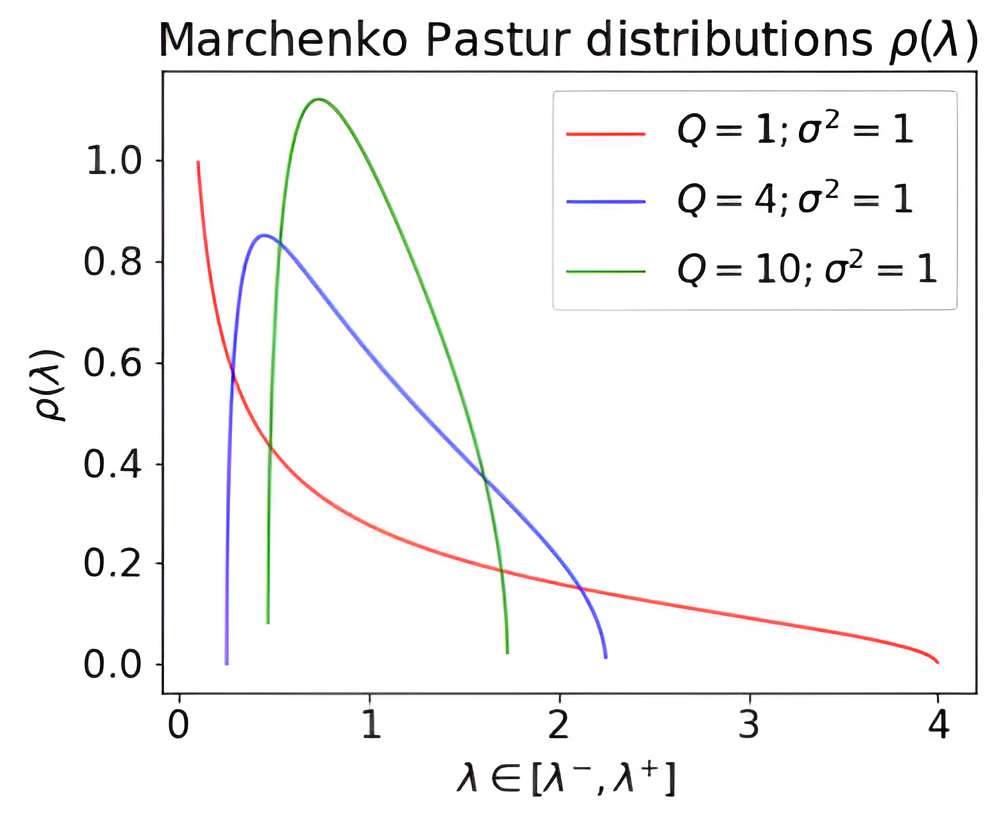
\includegraphics[width=0.5\linewidth]{img/marchenku-pastor.png}
    \caption[Ejemplos de distribuciones de Marchenko-Pastur~\cite{Charles2018}.]{Ejemplos de distribuciones de Marchenko-Pastur~\cite{Charles2018} para distintos valores de la relación de aspecto de la matriz ($Q = \frac{N}{P}$) y varianza fija. Cuando $Q = 1$, la mayoría de valores propios se acumulan alrededor del cero. A medida que $Q$ aumenta, los valores propios mínimos se alejan progresivamente de cero.}\label{fig:marchenkopastur}
\end{figure}

Por tanto, esos tres términos, multiplicados, determinan cuánto contribuye la $r$-ésima componente singular al error de predicción. Además, el ``pico'' del primer ascenso ocurre cerca del umbral de interpolación, debido a que el menor valor singular no nulo suele alcanzar su valor más bajo en dicho umbral, basado en la distribución de Marchenko-Pastur~\cite{Marchenko1967}.\newline

A grandes rasgos, esta distribución describe el comportamiento de los valores propios de matrices aleatorias y se aplica cuando se tiene una matriz aleatoria cuyas entradas son independientes e idénticamente distribuidas, como es el caso de la matriz $X \in \mathcal{M}_{N \times D}(\mathbb{R})$. En particular, la distribución de Marchenko-Pastur describe los valores propios de la matriz de covarianza $XX^{T}$, que a su vez determinan la varianza explicada por las componentes principales del modelo. De este modo, cuando la relación $\frac{N}{P}$ se aproxima a $1$, los valores propios más pequeños se acercan a $0$ (véase Figura~\ref{fig:marchenkopastur}), provocando que los valores singulares también sean casi nulos. Esto ocurre cerca del umbral de interpolación, donde $N = P = D$, y para evitar que el $N$-ésimo dato añada un valor singular pequeño no nulo a los datos de entrenamiento, deben cumplirse dos condiciones: 

\begin{itemize}
    \item Debe haber una dimensión en la que ninguno de los datos de entrenamiento anteriores haya variado significativamente.
    \item El $N$-ésimo dato debe presentar una variación considerable en esa dimensión.\newline
\end{itemize}

Sin embargo, este escenario es muy poco probable debido a que, en la mayoría de los casos, los datos de entrenamiento se muestrean de manera independiente a partir de variables aleatorias que son i.i.d., lo que resulta en una distribución aleatoria de los datos en todas las dimensiones. Al superar este umbral de interpolación, la varianza explicada por cada dimensión de las covariables se hace más evidente y los valores singulares no nulos más pequeños se alejan de cero, lo que reduce nuevamente el término de varianza en las predicciones, pudiendo provocar el doble descenso.\newline

\section{Convergencia del descenso de gradiente}\label{sec:sesgo-implicito-descenso-gradiente}

En esta sección, de cara a profundizar en la intuición obtenida en la sección anterior, vamos a analizar la influencia de utilizar el descenso de gradiente como método de optimización en problemas de regresión y clasificación, dado que es uno de los métodos más utilizados para entrenar redes neuronales.

\subsection{Problema de regresión}\label{subsec:problema-regresion}
En primer lugar, nos centraremos en abordar un problema de regresión utilizando el descenso de gradiente (basándonos en~\cite{Lafon2024}), en lugar de utilizar la solución que nos ofrece el problema de mínimos cuadrados asociado. Para ello, vamos a considerar nuevamente un problema de mínimos cuadrados bajo los mismos supuestos de la sección anterior. Por tanto, suponemos que nuestro conjunto de entrenamiento $\mathcal{D}$ está formado por $N$-pares de la forma $(x, y)$, donde $x \in \mathbb{R}^{D}$ y $y \in \mathbb{R}$. Así, nuestro conjunto de entrenamiento presenta la siguiente forma:

\[
    \mathcal{D} = \{ (x_i, y_i) \in \mathbb{R}^{D} \times \mathbb{R} \}, \; i \in \{ 1, \ldots, N \}.
\]\newline

Definimos $X \in \mathcal{M}_{N \times D}(\mathbb{R})$ como la matriz cuyas filas son los vectores $x_{i}^{T}$ e $y \in \mathbb{R}^{N}$ como el vector columna cuyos elementos son los $y_i$. Recordemos que la regla de actualización del descenso de gradiente para el vector de parámetros $w$, utilizando la función de pérdida $\mathcal{L}$ y una tasa de aprendizaje $\eta$, viene dada por:

\begin{equation}
    \mathbf{w}^{(\tau + 1)} = \mathbf{w}^{(\tau)} - \eta \nabla \mathcal{L}(\mathbf{w}).
    \label{eq:descenso-gradiente2}
\end{equation}\newline

De manera similar a la sección anterior, consideramos el siguiente problema de optimización para resolver la regresión lineal:

\begin{equation}\label{eq:regresion-lineal-gd}
    \min_{w \in \mathbb{R}^{D}} \mathcal{L}(w) = \min_{w \in \mathbb{R}^{D}} \frac{1}{2}\| Xw - y \|^{2}
\end{equation}

donde en la Ecuación~\eqref{eq:regresion-lineal-gd} se agrega el término $\frac{1}{2}$ para simplificar los cáculos de las derivadas en pasos posteriores. De esta forma, podemos enfocarnos en analizar las propiedades de la solución que encuentra el descenso de gradiente.\newline

\begin{teorema}
    El conjunto de soluciones de un problema de mínimos cuadrados, denotado por $\mathcal{S}_{LS}$, es exactamente el siguiente:

    \[
        \mathcal{S}_{LS} = \{ X^{\dagger}y + (I_D -X^{\dagger}X)u, \; u \in \mathbb{R}^{D} \}.
    \]
\end{teorema}

\begin{proof}
    Podemos expresar el error de la Ecuación~\eqref{eq:regresion-lineal-gd} de la siguiente forma: $Xw - y = Xw - XX^{\dagger}y +XX^{\dagger}y - y = Xw - XX^{\dagger}y - (I_D - XX^{\dagger})y$.\newline

    A partir de la última ecuación, sabemos que $XX^{\dagger}y$ representa la proyección de $y$ sobre el espacio columna de $X$ y $(I_D - XX^{\dagger})y$ corresponde a su componente ortogonal. Esto se debe a que $XX^{\dagger}y$ es la proyección sobre $Im(X)$ y $(I_D - XX^{\dagger})y$ es la proyección en el complemento ortogonal de $Im(X)$, es decir, el $\ker(X^{T})$. Para verificar estas afirmaciones, basta utilizar ambas propiedades de manera conjunta en el Lema~\ref{lema:propiedades-pseudoinversa}.\newline

    Dado que ambos términos son ortogonales, podemos descomponer la norma del error de la siguiente forma:

    \[
        \| Xw - y \|^{2} = \| Xw - XX^{\dagger}y \|^{2} + \| (I_D - XX^{\dagger})y \|^{2}
    \]

    lo que nos lleva a la siguiente desigualdad:

    \[
        \| Xw - y \|^{2} \geq \| (I_D - XX^{\dagger})y \|^{2}.
    \]

    Finalmente, la igualdad se alcanza si y solo si:

    \[
        Xw - XX^{\dagger}y = 0 \implies  Xw = XX^{\dagger}y.
    \]

    De esta manera, sabemos que $X^{\dagger}y$ es una solución particular de la ecuación $Xw = XX^{\dagger}y$. Para obtener la solución general, basta con añadir cualquier vector que se encuentre en el núcleo de $X$, es decir, cualquier vector de la forma $\{ (I_D-X^{\dagger}X)u, \; u \in \mathbb{R}^{D} \}$ (véase Lema~\ref{lema:propiedades-pseudoinversa}).\newline
\end{proof}

Una vez que conocemos el conjunto de soluciones para nuestro problema de optimización, podemos analizar cómo se comporta dicho conjunto en función del rango de la matriz $X$.

\begin{observacion}
    Dependiendo del rango de la matriz $X$, el conjunto de soluciones $\mathcal{S}_{LS}$ variará en función de la expresión de la pseudoinversa $X^{\dagger}$:

    \begin{itemize}
        \item Si $N < D$ y $rang(X) = N$, entonces $X^{\dagger} = X^{T}{(XX^{T})}^{-1}$ y $\mathcal{S}_{LS} = \{ X^{T}{(XX^{T})}^{-1}y + (I_D-X^{T}{(XX^{T})}^{-1}X)u, \; u \in \mathbb{R}^{D} \}$.
        
        \item Si $D < N$ y $rang(X) = D$, entonces $X^{\dagger} = {(X^{T}X)}^{-1}X^{T}$ y $\mathcal{S}_{LS} = \{ {(X^{T}X)}^{-1}X^{T}y \}$.
        
        \item Si $D = N$ y $X$ tiene inversa, entonces $X^{\dagger} = {X}^{-1}$ y $\mathcal{S}_{LS} = \{{X}^{-1}y \}$.
    \end{itemize}

    En particular, en los dos últimos casos, dado que $\ker(X)$ es trivial, la solución del problema es única.\newline
\end{observacion}

Por tanto, nos interesa centrarnos en analizar qué tan buena es la solución que proporciona el descenso de gradiente en la región sobreparametrizada, es decir, cuando $N < D$, dado que es en este caso cuando se generan múltiples soluciones, mientras que en los otros casos la solución es única.

\begin{teorema}
    Si el problema de mínimos cuadrados lineales~\eqref{eq:regresion-lineal-gd} se encuentra en la región sobreparametrizada, es decir, $(N < D)$ y $rang(X) = N$, entonces, usando el descenso de gradiente con una tasa de aprendizaje constante $0 < \eta < \frac{1}{\lambda_{\max}(X)}$, donde $\lambda_{\max}(X)$ es el mayor valor propio de $X$ y partiendo desde un punto inicial $w_0 \in Im(X^{T})$, se garantiza la convergencia hacia la solución de norma mínima.
\end{teorema}

\begin{proof}
    Dado que estamos suponiendo que $X$ tiene $N$ filas linealmente independientes, podemos expresar su descomposición en valores singulares de la siguiente manera:

    \[
        X = U \Sigma V^T = \begin{bmatrix} U_1 & U_2 \end{bmatrix} \begin{bmatrix} \Sigma_1 & 0 \\ 0 & 0 \end{bmatrix} \begin{bmatrix} V_1^T \\ V_2^T \end{bmatrix}
    \]

    donde $U \in \mathbb{R}^{N \times N}$ y $V \in \mathbb{R}^{D \times D}$ son matrices ortogonales, $\Sigma \in \mathbb{R}^{N \times D}$ es una matriz diagonal rectangular, $U_1$ (respectivamente $V_1$) son las submatrices que contienen los vectores singulares izquierdos (respectivamente derechos) asociados con los valores singulares no nulos y $\Sigma_1 \in \mathbb{R}^{n \times n}$ es una matriz diagonal con valores singulares no nulos.\newline

    Nos centramos ahora en encontrar la solución de norma mínima $w^{*}$, la cual, como sabemos, viene dada por la pseudoinversa:

    \[
        w^* = X^T {(X X^T)}^{-1} y.
    \]\newline

    Utilizando la descomposición en valores singulares de las matrices $X$ y $X^{T}$, y dado que $V$ es ortogonal, obtenemos:

    \[
        X X^T = U \Sigma V^{T} V \Sigma^{T} U^{T} = U \Sigma \Sigma^{T} U^{T}.
    \]\newline

    Así, para la inversa de la matriz ${(X X^T)}$, sabiendo que $U$ es ortogonal, nos queda:

    \[
        {(X X^T)}^{-1} = U {(\Sigma \Sigma^{T})}^{-1} U^{T}.
    \]\newline

    Volviendo a usar la descomposición en valores singulares para la matriz $X^{T}$, $X^{T} = V \Sigma U^{T}$, obtenemos que la solución de norma mínima $w^{*}$ se puede reescribir como sigue (los vectores singulares asociados a los valores singulares nulos no tienen impacto en la solución de mínimos cuadrados, pues su dirección es linealmente dependiente):

    \[
        w^* = X^T {(X X^T)}^{-1} y = V \Sigma U^{T} U {(\Sigma \Sigma^{T})}^{-1} U^{T}y = V_1 \Sigma_1^{-1} U_{1}^T y.
    \]\newline

    A continuación, trabajamos sobre la regla de actualización del gradiente descendente, que viene dada por:
    \[
        w^{(k+1)} = w^{(k)} - \eta \nabla \mathcal{L}(w) = w^{(k)} - \eta X^T (Xw^{(k)} - y) = (I - \eta X^T X)w^{(k)} + \eta X^T y
    \]

    donde $X^T (Xw^{(k)} - y)$ hace referencia a la derivada de $\mathcal{L}(w)$ respecto de $w$.\newline

    Seguidamente, aplicando inducción, obtenemos la expresión general:
    \[
        w^{(k)} = (I - \eta X^T X)^k w_0 + \eta \sum_{l=0}^{k-1} (I - \eta X^T X)^l X^T y.
    \]\newline


    Ahora bien, usando la descomposición en valores singulares para la matriz $X^T X$ $(V \Sigma^T \Sigma V^T)$ y dado que $V$ es ortogonal, la iteración del gradiente descendente para el paso $k$-ésimo se expresa como:
    \[
        w^{(k)} = V (I - \eta \Sigma^T \Sigma)^k V^T w_0 + \eta V \left(\sum_{l=0}^{k-1} (I - \eta \Sigma^T \Sigma)^l \Sigma^T \right)U^T y.
    \]\newline

    Reescribiendo la ecuación anterior en términos de $\Sigma_1$, obtenemos:
    \[
        w^{(k)} = V \begin{bmatrix} (I - \eta \Sigma_1^2)^k & 0 \\ 0 & I \end{bmatrix} V^T w_0 + \eta V \left(\sum_{l=0}^{k-1} \begin{bmatrix} (I - \eta \Sigma_1^2)^l \Sigma_1 \\ 0 \end{bmatrix} \right) U^T y.
    \]

    De cara a garantizar la convergencia del descenso de gradiente, elegimos $0 < \eta < \frac{1}{\lambda_{\max}(\Sigma_1)}$, lo que asegura que los valores propios de $I - \eta \Sigma^T \Sigma$ sean estrictamente menores que $1$, lo que implica, a su vez, que:

    \[
        \left( I - \eta \Sigma_1^T \Sigma_1 \right)^k \to 0 \quad \text{cuando} \quad k \to \infty
    \]

    y, por tanto,

    \[
        V \begin{bmatrix} (I - \eta \Sigma_1^2)^k & 0 \\ 0 & I \end{bmatrix} V^T w_0 \xrightarrow{k \to \infty} V \begin{bmatrix} 0 & 0 \\ 0 & I \end{bmatrix} V^T w_0 = V_2 V_2^T w_0
    \]\newline

    dado que $V_{2}^{T}w_0$ es la parte de $w_0$ correspondiente a los valores singulares nulos de $X^{T}X$.\newline

    Además,
    \[
        \eta \sum_{l=0}^{k-1} \begin{bmatrix} (I - \eta \Sigma_1^2)^l \Sigma_1 \\ 0 \end{bmatrix}  \xrightarrow{k \to \infty} \eta \begin{bmatrix} \sum_{l=0}^{\infty}(I - \eta \Sigma_1^2)^l \Sigma_1 \\ 0 \end{bmatrix} = \begin{bmatrix} \eta(I - I + \eta \Sigma_1^2)^{-1} \Sigma_1 \\ 0 \end{bmatrix} = \begin{bmatrix} \Sigma_1^{-1} \\ 0 \end{bmatrix}
    \]\newline

    Por consiguiente, denotando $w_\infty$ como el límite de las iteraciones del gradiente descendente, obtenemos:
    \[
        w_\infty = V_2 V_2^T w_0 + V_1 \Sigma_1^{-1} U^T y = V_2 V_2^T w_0 + X^{T}{(XX^{T})}^{-1}y = V_2 V_2^T w_0 + w^*.
    \]\newline

    Finalmente, dado que $w_0$ está en la imagen de $X^T$, podemos escribir $w_0 = X^T z$ para algún $z \in \mathbb{R}^N $, lo que implica (usando la descomposición en valores singulares de la matriz $X^{T}$):
    \[
        V_2 V_2^T w_0 = V \begin{bmatrix} 0 & 0 \\ 0 & I \end{bmatrix}V^{T}X^{T}z = V \begin{bmatrix} 0 & 0 \\ 0 & I \end{bmatrix}V^{T}V\Sigma^{T}U^{T}z = V \begin{bmatrix} 0 & 0 \\ 0 & I \end{bmatrix}\begin{bmatrix} \Sigma_1 \\ 0 \end{bmatrix}U^{T} = 0.
    \]\newline

    En consecuencia, el término $V_2 V_2^T w_0$ desaparece, y nos queda que $w_\infty = w^{*}$, por lo que el gradiente descendente converge a la solución de norma mínima.\newline
\end{proof}

En conclusión, tanto el gradiente descendente como la pseudoinversa llegan a la misma solución (bajo ciertas hipótesis) cuando se trata de resolver un problema de regresión lineal, ya que ambos buscan la solución interpolante de norma mínima, lo que los convierte en métodos equivalentes. De esta manera, realizar el gradiente descendente hasta la convergencia, comenzando con una inicialización de todos los pesos a cero, es equivalente a aplicar directamente la pseudoinversa. Por tanto, podemos interpretar que utilizar la pseudoinversa para resolver un problema de mínimos cuadrados es, en esencia, un caso particular del gradiente descendente aplicado al mismo problema.\newline

\subsection{Problema de clasificación con datos separables}\label{subsec:problema-clasificación-separable}
En esta subsección, nos preocupamos de verificar el efecto de utilizar el descenso de gradiente como método de optimización en un problema de clasificación binaria con un conjunto de datos linealmente separable~\cite{Soudry2024}. Por simplicidad, condideramos un problema de clasificación binaria con un dataset separable, lo que facilita la intuición sobre el comportamiento del descenso de gradiente. No obstante, los principios que se discuten posteriormente pueden extenderse a problemas de clasificación multiclase~\cite{Ravi2024} y al uso del descenso de gradiente en redes neuronales~\cite{Gunasekar2019}.\newline

\begin{definicion}
    Un conjunto de datos $\mathcal{D} = \{ (x_i, y_i) \; | \; i \in \{1, \ldots, N \}\}$ donde para todo $i \in \{1, \ldots, N \}$ se verifica que $(x_i, y_i) \in \mathbb{R}^{D} \times \{-1, 1\}$, es linealmente separable si existe $w_{*} \in \mathbb{R}^{D}$ de manera que $\forall i : y_i w_{*} x_i > 0$.\newline
\end{definicion}

Además, los resutados que se exponen en este apartado se cumplen para funciones de pérdida $\ell: \mathbb{R} \to \mathbb{R}_{+}$ que presentan las siguientes propiedades:
\begin{enumerate}
    \item\label{prop:positiva} $\ell$ es positiva, diferenciable y decreciente de manera monótona a cero $(\ell(u)>0, \ell'(u)<0 \; \text{y} \; \lim \limits_{u \to \infty} \ell(u) = \lim \limits_{u \to \infty} \ell'(u) = 0)$.
    \item\label{prop:smooth} $\ell$ es una función $\beta$-suave, es decir, el gradiente de $\ell$ es $\beta$-Lipschitz $(\forall u,v \in \mathbb{R}, \; \| \nabla \ell(u) - \nabla \ell(v) \| \leq \beta \| u-v \|)$.
    \item\label{prop:derivada_negativa} $\lim \limits_{u \to -\infty} \ell'(u) < 0$.\newline
\end{enumerate}

Estas propiedades incluyen funciones de pérdida comunes para problemas de clasificación binaria, incluyendo la función logística y la exponencial. Además, estas propiedades implican que $\mathcal{L}(w)$ es una función $\beta \sigma^{2}_{\max}(X)$-suave (ligado al hecho de que $\ell$ es $\beta$-suave), donde $\sigma_{\max}(X)$ es el máximo valor singular de la matriz $X \in \mathbb{R}^{D \times N}$ que contiene los datos de entrenamiento.\newline

Por tanto, para nuestro problema, consideramos un conjunto de entrenamiento $\mathcal{D}$ linealmente separable formado por $N$-pares de datos de la forma $(x_i, y_i)$ con $x_i \in \mathbb{R}^{D}$ y $y_i \in \{ -1, 1\}$, donde $i \in \{1, \ldots, N \}$ y nos centramos en minimizar la función de pérdida dada por:

\[
    \min_{w \in R^{D}}\mathcal{L}(w) = \min_{w \in R^{D}} \sum_{i=1}^{N} \ell(y_i w^{T}x_i)
\]

donde $w \in \mathbb{R}^{D}$ es el vector de parámetros y $\ell$ es una función de pérdida binaria verificando las propiedades~\ref{prop:positiva},~\ref{prop:smooth} y~\ref{prop:derivada_negativa} descritas anteriormente.\newline

Seguidamente, nos ocupamos de estudiar la solución que ofrece el descenso de gradiente para este problema, fijada una tasa de aprendizaje $\eta$:

\[
    \mathbf{w}^{(\tau + 1)} = \mathbf{w}^{(\tau)} - \eta \nabla \mathcal{L}(\mathbf{w}) = \mathbf{w}^{(\tau)} - \eta \sum_{i=1}^{N} \ell'(y_i w^{T}x_i)y_i x_i.
\]\newline

De cara a estudiar esta solución, utilizaremos un lema auxiliar que nos ayudará con la demostración del resultado principal de esta subsección.
\begin{lema}\label{lema:raro-clasificación-gd}
    Sea $\mathcal{L}(w)$ una función $\beta$-suave no negativa. Si $\eta < \frac{2}{\beta}$, entonces, para cualquier $w_0$ y utilizando el método del descenso de gradiente dado por:

    \[
        w^{(\tau + 1)} = w^{(\tau)} - \eta \nabla \mathcal{L}(w)
    \]

    se tiene que $\sum_{u=0}^{\infty} \| \nabla\mathcal{L}(w^{(u)}) \|^{2} < \infty$ y, por tanto:

    \[
        \lim \limits_{t \to \infty} \| \nabla\mathcal{L}(w^{(t)}) \|^{2} = 0.
    \]
\end{lema}

La demostración del lema se puede verificar en el Apéndice~\ref{ap:apendiceA}.\newline

Una vez conocemos el resultado anterior, podemos enunciar el principal teorema de esta subsección, que establece las condiciones necesarias para que el descenso de gradiente converja hacia un punto crítico.

\begin{teorema}\label{teorema:clasificación-gd}
    Sea $\mathcal{D}$ un conjunto de entrenamiento linealmente separable con $N$ ejemplos y $\ell: \mathbb{R} \to \mathbb{R}_{+}$ una función de pérdida verificando las propiedades~\ref{prop:positiva},~\ref{prop:smooth} y~\ref{prop:derivada_negativa}. Sean $w_t$ las iteraciones del descenso de gradiente usando una tasa de aprendizaje $0 < \eta < \frac{2}{\beta \sigma^{2}_{\max}(X)}$ y cualquier punto inicial $w_0$. Entonces, se cumplen:

    \begin{enumerate}
        \item $\lim \limits_{t \to \infty} \mathcal{L}(w^{(t)}) = 0$.
        \item $\lim \limits_{t \to \infty} \| w^{(t)} \| = \infty$.
        \item $\forall i \in \{ 1, \ldotp, N\}: \; \lim \limits_{t \to \infty} y_i {w}^{(t)T} x_i = \infty$.
    \end{enumerate}
\end{teorema}

\begin{proof}
    Dado que el conjunto de entrenamiento $\mathcal{D}$ es linealmente separable, $\exists w_{*} \in \mathbb{R}^{D}$ de manera que $\forall i \in \{1, \ldots, N \} : y_i w_{*} x_i > 0$ y, entonces

    \[
        w_{*}^{T}\nabla\mathcal{L}(w) = \sum_{i=1}^{N} \underbrace{\ell'(y_i w^{T} x_i)}_{< 0} \underbrace{y_i w_{*}^{T}x_i}_{> 0} < 0.
    \]

    Para cualquier $w$ finito, la suma anterior no puede ser igual a $0$, ya que es una suma de términos negativos $(\forall i: y_i w_{*}^{T}x_i > 0)$ y $\forall u: \ell'(u) < 0$, debido a las propiedades que cumple la función de pérdida $\ell$. Por lo tanto, no hay puntos críticos finitos $w$ para los cuales $\nabla \mathcal{L}(w) = 0$. Sin embargo, el descenso de gradiente en una función de pérdida suave con una tasa de aprendizaje adecuada siempre garantiza converger a un punto crítico, es decir, $\nabla \mathcal{L}(w^{(t)}) \to 0$ (véase Lema~\ref{lema:raro-clasificación-gd}).\newline
    
    Este hecho implica necesariamente que $\| w^{(t)} \| \to \infty$, que es la condición \textbf{(2)}, mientras se verifique que $\exists t_0 : \; \forall t > t_0, \; \forall i: y_i w_{t}^{T} x_i > 0$, que es la condición \textbf{(3)}, pues únicamente entonces se cumple $\ell'(y_i {w}^{(t)T} x_i) \to 0$. Entonces, se verifica que $\mathcal{L}(w^{(t)}) \to 0$ (condición \textbf{(1)}) y, por tanto, el descenso de gradiente converge hacia un mínimo global.\newline
\end{proof}

El Teorema~\ref{teorema:clasificación-gd} nos asegura que el descenso de gradiente, eligiendo una tasa de aprendizaje adecuada, converge hacia un mínimo global, dado que $\mathcal{L}(w^{(t)}) \to 0$. Además, no se requiere que la función de pérdida $\mathcal{L}(w)$ sea convexa, lo que amplia la aplicabilidad del resultado a una clase más general de funciones.\newline

\section{Optimización en la zona sobreparametrizada}\label{sec:optimizacion-zona-sobreparametrizada}

Como hemos observado en secciones anteriores, la sobreparametrización resulta beneficiosa dentro del marco del aprendizaje estadístico. Este comportamiento, aunque contraintuitivo como se indica en~\cite{Hastie2001}, que afirma: ``Un modelo con error de entrenamiento cero sobreajusta los datos de entrenamiento y, por lo general, generalizará mal'', refleja cómo las soluciones de los sistemas sobreparametrizados pueden mejorar la generalización.\newline

Como hemos observado en secciones anteriores, la sobreparametrización resulta beneficiosa dentro del marco del aprendizaje estadístico. Este comportamiento, aunque contraintuitivo~\cite{Hastie2001} ``Un modelo con cero error de entrenamiento está por encima de los datos de entrenamiento y, por lo general, generalizará mal'', refleja cómo las soluciones de los sistemas sobreparametrizados pueden mejorar la generalización. Sin embargo, desde el punto de vista de la optimización, que se concentra en los algoritmos y técnicas utilizadas para encontrar el mejor modelo posible, la sobreparametrización también ofrece ventajas, ya que facilita la convergencia de los métodos de optimización hacia un mínimo global, especialmente en aquellos que emplean el descenso de gradiente o alguna extensión del mismo.\newline

En el caso de que nuestra función de pérdida $\ell: \mathcal{Y} \to \mathbb{R}$ sea convexa y nuestro modelo $g: \mathcal{X} \to \mathcal{Y}$, elegido del conjunto de hipótesis, sea lineal, es fácil observar que $l \circ f$ es convexa (basta con aplicar las propiedades de la linealidad de $g$ junto con las propiedades de convexidad de $\ell$). Como resultado, se garantiza la convergencia hacia la mejor solución, es decir, el mínimo global de la función de pérdida, sin riesgo de quedar atrapados en mínimos locales.\newline

No obstante, en el marco del aprendizaje profundo, el modelo resultante es no lineal debido al uso de funciones de activación no lineales, lo que provoca que, en general, el paisaje de la función de pérdida sea no convexo. Esto implica que los métodos de optimización de primer orden, como el GD, puedan quedar atrapados en mínimos locales, ya que solo utilizan información local del gradiente, dependiendo así de su inicialización. Como resultado, los sistemas sobreparametrizados dan lugar a paisajes de la función de pérdida que son \textit{esencialmente no convexos}, es decir, por lo general no existe un vecindario alrededor de ningún minimizador global en el que el paisaje de la función de pérdida sea convexo. Esto contrasta con lo que ocurre en los sistemas infraparametrizados, donde dicho vecindario suele existir, aunque sea extremadamente pequeño (véase Figura~\ref{fig:localglobalminima}).\newline

\begin{figure}[h]
    \centering
    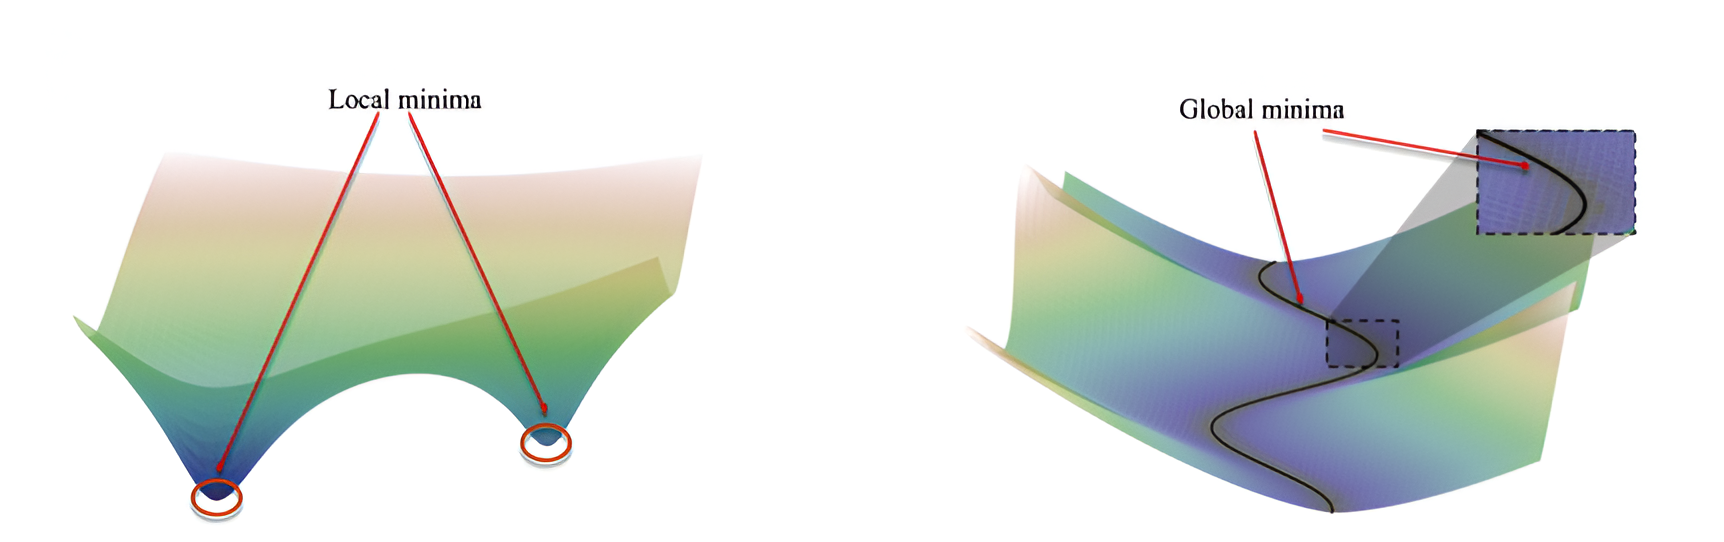
\includegraphics[width=0.8\linewidth]{img/localglobalminima.png}
    \caption[Ejemplos de paisajes de la función de pérdida en redes neuronales~\cite{Liu2021}.]{Ejemplos de paisajes de la función de pérdida en redes neuronales~\cite{Liu2021}. A la izquierda, se muestra un paisaje localmente convexo alrededor de los mínimos locales, ligado a la zona infraparametrizada. A la derecha, se muestra un paisaje incompatible con la convexidad local con múltiples mínimos globales, ligado a la zona sobreparametrizada.}\label{fig:localglobalminima}
\end{figure}

Con el fin de estudiar de manera más formal los resultados presentados, consideramos nuevamente un problema típico del aprendizaje supervisado, con un dataset $\mathcal{D}$ compuesto por $N$-pares de ejemplos de entrenamiento, es decir,  $\mathcal{D} = \{(x_i, y_i)\}_{1}^{N}$, con $x_i \in \mathbb{R}^{D}$ e $y \in \mathbb{R}$. Si consideramos nuestro conjunto de hipótesis $\mathcal{H}$ como una familia paramétrica de modelos, como, por ejemplo, una red neuronal, nuestro objetivo es encontrar el vector de parámetros óptimo $w^{*}$, de manera que el modelo se ajuste a los datos de entrenamiento, es decir

\[
    f(w^{*}; x_i) \approx y_i, \quad i \in \{1,\ldots,n \}.
\]

Matemáticamente, esto es equivalente a resolver un sistema con $N$ ecuaciones\footnote{Para problemas de clasificación multiclase o problemas de regresión con múltiples salidas, donde $C$ es el número de clases o salidas distintas, estaremos resolviendo un sistema de $N \times C$ ecuaciones.}. Agregándolas todas en una única función, podemos escribir:

\begin{equation}\label{eq:optimizacion-uno}
    \mathcal{F}(w) = y, \; \text{donde} \; w \in \mathbb{R}^{P}, y \in \mathbb{R}^{N}, \mathcal{F}(\cdot):\mathbb{R}^{P} \to \mathbb{R}^{N}.
\end{equation}

De esta manera, $(\mathcal{F}(w)) = f(w; x_i)$. Una solución exacta de la Ecuación~\eqref{eq:optimizacion-uno} corresponde a la interpolación.\newline

Usamos $\mathcal{DF}$ para representar la derivada de la función $\mathcal{F}$, donde $\mathcal{DF} \in \mathcal{M}_{N \times P}(\mathbb{R})$, con $(\mathcal{DF})_{ij} = \frac{\partial \mathcal{F}_{i}}{\partial w_j}$. Denotamos la matriz hessiana de la función $\mathcal{F}$ como $H_{\mathcal{F}}$, que es un tensor de tamaño $N \times P \times P$ con $(H_{\mathcal{F}})_{ijk} = \frac{\partial^2 \mathcal{F}_{i}}{\partial w_j \partial w_k}$, y definimos la norma del tensor hessiano como $\| H_{\mathcal{F}} \| = \max_{i \in \{1, \ldots,N \}} \| H_{\mathcal{F}_{i} \|}$, donde $H_{\mathcal{F}_{i}} = \frac{\partial^2 \mathcal{F}_{i}}{\partial w^2}$. De manera análoga, denotamos la matriz hessiana de la función de pérdida como $H_{\mathcal{L}} = \frac{\partial^2 \mathcal{L}}{\partial w^2}$.\newline

Para detallar de manera analítica la no convexidad en la zona sobreparametrizada, se presenta el siguiente resultado.

\begin{proposicion}\label{prop:non-conexity}
    Sea $w^{*}$ una solución, es decir, $\mathcal{L}(w^{*}) = 0$, y supongamos que $\frac{d}{dw}\frac{\partial \mathcal{L}}{\partial \mathcal{F}}(w^{*}) \neq 0$ y $rang(H_{\mathcal{F}_{i}}(w^{*})) > 2N$ para algún $i \in \{1, \ldots, N \}$. Entonces $\mathcal{L}(w)$ no es convexa en ninguna vecindad de $w^{*}$.
\end{proposicion}

\begin{proof}
    Se presenta una idea intuitiva de cómo realizar la demostración del resultado anterior. Para ello, tomaremos dos puntos distintos del vecindario de la solución $w^*$ y evaluaremos las matrices hessianas de la función de pérdida en dichos puntos. Una vez evaluadas, podemos verificar que alguna de las matrices anteriores es no negativa, lo que implica que la función de pérdida $\mathcal{L}(w)$ no es localmente convexa alrededor de $w^*$, ya que la hessiana no es semidefinida positiva en esa vecindad, lo cual es una condición necesaria para que la función sea localmente convexa.\newline

    Por último, se referencia al lector más curioso al Apéndice~\ref{ap:apendiceA} para la demostración detallada de la proposición.\newline
\end{proof}

Para el caso de sistemas infraparametrizados, los mínimos locales se encuentran generalmente aislados. Dado que $H_{\mathcal{L}}(w^{*})$ es definida positiva cuando $w^{*}$ es un mínimo aislado, por la continuidad de $H_{\mathcal{L}}(\cdot)$, la definición de positivad se preserva en la vecindad de $w^{*}$. Por consiguiente, $\mathcal{L}(w)$ es localmente convexa alrededor de $w^{*}$.\newline

A su vez, en los sistemas sobreparametrizados contamos con más parámetros que constantes. En este caso, el sistema de ecuaciones general tiene múltiples soluciones exactas, las cuales forman una variedad continua de dimensión $P - N > 0$, de modo que ninguna de estas soluciones está aislada. Este hecho puede observarse en la Figura~\ref{fig:localglobalminima} y se encuentra demostrado en el Apéndice A de~\cite{Liu2021}. En cuanto a nuestro interés, podemos concluir que, para redes suficientemente parametrizadas, los mínimos globales siempre están rodeados por otro mínimo global en un vecindario relativamente pequeño.\newline

Estos resultados nos conducen a la conclusión de que, para el análisis de los sistemas sobreparametrizados, no podemos utilizar la convexidad, ni siquiera localmente, como base. En consecuencia, es necesario buscar una condición, a priori, más simple, que verifiquen las funciones de pérdida con el fin de analizar el comportamiento de dichos sistemas. Para ello, se recurre a una modificación de la condición de Polyak y Lojasiewicz.\newline

\begin{definicion}[Condición $\mu$-$PL$]
    Decimos que una función no negativa $\mathcal{L}$ verifica la condición $\mu$-$PL$ (Polyak-Lojasiewicz) en un conjunto $\mathcal{S} \subset \mathbb{R}^{P}$ para $\mu > 0$, si

    \[
        \| \nabla \mathcal{L}(w) \|^{2} \geq \mu \mathcal{L}(w), \; \forall w \in \mathcal{S}.
    \]\newline
\end{definicion}

\begin{teorema}
    Supongamos que la función de pérdida $\mathcal{L}(w)$ es $\beta$-suave y cumple la condición $\mu$-$PL$ en la bola $B(w_0, R) = \{ w \in \mathbb{R}^{P} : \| w - w_0 \| \leq R \}$ con $R = \frac{2 \sqrt{2 \beta \mathcal{L}(w_0)}}{\mu}$. Entonces se tiene:

    \begin{enumerate}
        \item (\textbf{Existencia de una solución}). Existe una solución (minimizador global de $\mathcal{L}$) $w^{*} \in B(w_0, R)$, de manera que $\mathcal{F}(w^{*}) = y$.
        \item (\textbf{Convergencia del GD}). El gradiente descendente con un learning rate $\eta \leq \frac{1}{\sup_{w \in B(w_0, R)} \| \mathcal{H}_{\mathcal{L}}(w) \|}$ converge a una solución global en $B(w_0, R)$.
    \end{enumerate}
\end{teorema}

\begin{proof}
    Probaremos este teorema por inducción, sabiendo que nuestra hipótesis de inducción nos dice que, para todo $t \geq 0$, $w_t$ está dentro de la bola $B(w_0, R)$ con $R = \frac{2\sqrt{2\beta \mathcal{L}(w_0)}}{\mu}$.\newline

    En el caso inicial, cuando $t = 0$, es trivial que $w_0 \in B(w_0, R)$. Supongamos que, por inducción, para un $t \geq 0$, $w_t$ está en la bola $B(w_0, R)$. Para probar que $w_{t+1} \in B(w_0, R)$, usando que la función de pérdida $\mathcal{L}$ es $\beta$-suave, tenemos que:
    \begin{align}
        \| w_{t+1} - w_0 \| &= \eta \bigg\| \sum_{i=0}^{t} \nabla \mathcal{L}(w_i) \bigg\| \\
        &\leq \eta \sum_{i=0}^{t} \| \nabla \mathcal{L}(w_i) \| \\
        &\leq \eta \sum_{i=0}^{t} \sqrt{2 \beta (\mathcal{L}(w_i) - \mathcal{L}(w_{i+1}))} \\
        &\leq \eta \sum_{i=0}^{t} \sqrt{2 \beta \mathcal{L}(w_i)} \\
        &\leq \eta \sqrt{2\beta} \left( \sum_{i=0}^{t} (1 - \eta \mu)^{i/2} \right) \sqrt{\mathcal{L}(w_0)} \\
        &\leq \eta \sqrt{2\beta} \sqrt{\mathcal{L}(w_0)} \frac{1}{1 - \sqrt{1 - \eta \mu}} \\
        &\leq \frac{2 \sqrt{2\beta} \sqrt{\mathcal{L}(w_0)}}{\mu} = R.
    \end{align}

    Por tanto, $w_{t+1}$ se encuentra en la bola $B(w_0, R)$.\newline
\end{proof}

Finalmente, se presenta una idea intuitiva, utilizando la función de pérdida cuadrática, de por que los paisajes de pérdida de los sistemas sobreparametrizados satisfacen la condición $\mu$-PL en la mayor parte de su espacio de parámetros.\newline

\begin{definicion}
    El núcleo tangente de la función $\mathcal{F}$ en el vector $w$ se define como

    \[
        K(w) = \mathcal{DF}(w)\mathcal{DF}^{T}(w)
    \]

    donde $K(w) \in \mathcal{M}_{N \times P}(\mathbb{R})$ es una matriz semidefinida positiva.\newline
\end{definicion}

\begin{definicion}[Condicionamiento uniforme]
    Decimos que $\mathcal{F}(w)$ está $\mu$-uniformemente condicionada $(\mu > 0)$ en un subconjunto $\mathcal{S} \subset \mathbb{R}^{P}$ si el valor propio más pequeño de su núcleo tangente satisface

    \[
        \lambda_{\min}(K(w)) \geq \mu, \; \forall w \in \mathcal{S}.
    \]\newline
\end{definicion}

El siguiente resultado muestra cómo el hecho de estar condicionada de manera uniforme es una condición suficiente para que la pérdida cuadrática cumpla la condición $\mu$-PL.

\begin{teorema}[Condicionamiento uniforme $\implies$ Condición $\mu$-PL]
    Si $\mathcal{F}(w)$ está $\mu$-uniformemente condicionada en un conjunto $\mathcal{S} \subset \mathbb{R}^P$, entonces la función de pérdida cuadrática $\mathcal{L}(w) = \frac{1}{2} \|\mathcal{F}(w) - y \|^2$ satisface la condición $\mu$-PL$^*$ en $\mathcal{S}$.
\end{teorema}

\begin{proof}
    \[
        \begin{aligned}
            \frac{1}{2} \|\nabla \mathcal{L}(w)\|^2 &= \frac{1}{2} (\mathcal{F}(w) - y)^T K(w) (\mathcal{F}(w) - y) \\
            &\geq \frac{1}{2} \lambda_{\min}(K(w)) \|\mathcal{F}(w) - y \|^2 = \lambda_{\min}(K(w)) \mathcal{L}(w) \geq \mu \mathcal{L}(w).
        \end{aligned}
    \]

\end{proof}

Nos centramos ahora en mostrar una intuición de por qué la pérdida cuadrática cumple la condición $\mu$-PL en la mayor parte del espacio de parámetros. La observación clave viene dada por el rango del núcleo tangente:

\[
        rang(K(w)) = rang((D\mathcal{F}(w) D\mathcal{F}^T(w))) = rang(D\mathcal{F}(w))
\]

donde $K(w)$ es, por definición, una matriz semidefinida positiva. Por tanto, el conjunto singular $\mathcal{S}_{\text{sing}}$, donde el núcleo tangente es degenerado, se puede escribir como

\[
    \mathcal{S}_{\text{sing}} = \{w \in \mathbb{R}^P \mid \lambda_{\min}(K(w)) = 0\} = \{w \in \mathbb{R}^P \mid \text{rango } D\mathcal{F}(w) < n\}.
\]

Así, tenemos que $rang(K(w)) = \min(P, N)$. Para el caso más simple, consideremos $N = 1$. En este caso, el núcleo tangente es un escalar y $K(w) = \| \mathcal{DF}(w) \|^2$ es singular si y solo si $D\mathcal{F}(w) = 0$. Como resultado, mediante un análisis de conteo de parámetros, esperamos que el conjunto singular $\mathcal{S}_{\text{sing}} = \{ w \mid K(w) = 0 \}$ tenga codimensión $P$ y, en consecuencia, consista únicamente de puntos aislados.\newline

\begin{figure}[h]
    \centering
    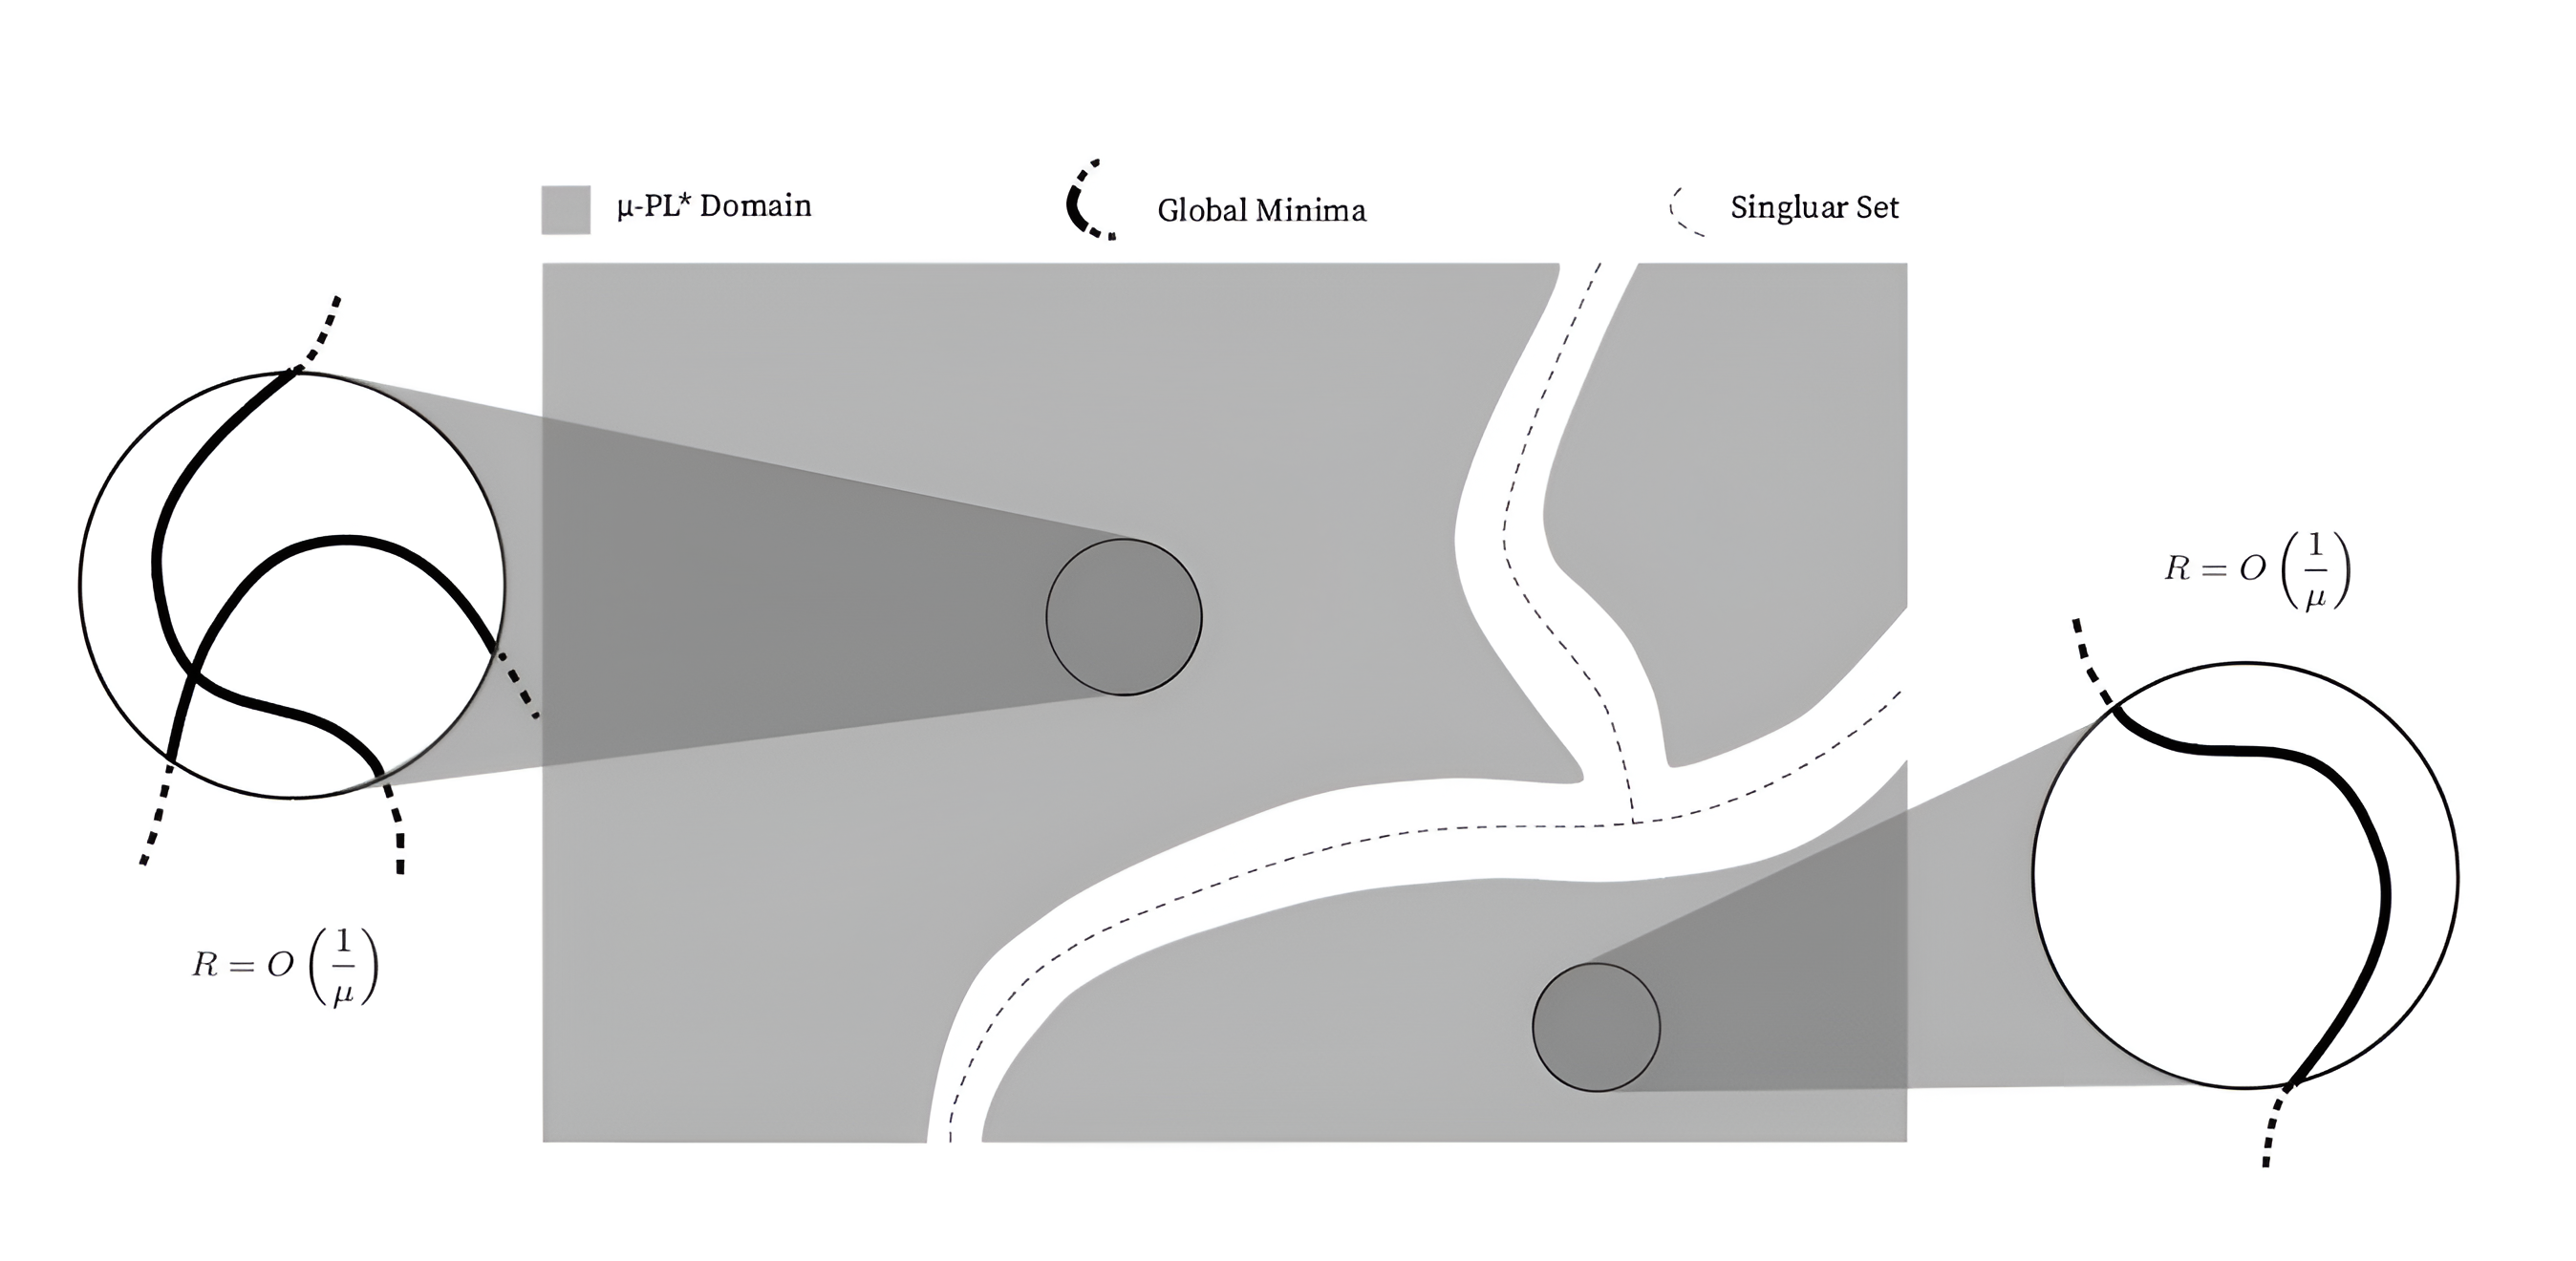
\includegraphics[width=0.8\linewidth]{img/cosarara2.png}
    \caption[Ejemplo de función de pérdida que satisface la condición $\mu$-PL~\cite{Liu2021}.]{Ejemplo de función de pérdida que satisface la condición $\mu$-PL~\cite{Liu2021}. La función de pérdida es $\mu$-PL en la zona sombreada. El conjunto singular corresponde a los vectores $w$ con núcleo tangente degenerado. Cada bola de radio $R = O\left(\frac{1}{\mu}\right)$ dentro del dominio $\mu$-PL se interseca con el conjunto de mínimos globales de la función de pérdida.}\label{fig:cosarara2}
\end{figure}

Aplicando un razonamiento similar, cuando $P > N$, esperamos que $\mathcal{S}_{\text{sing}}$ tenga codimensión positiva ($P - N + 1$) y sea un conjunto de medida cero. Esto significa que, dentro de un conjunto compacto, para valores suficientemente pequeños de $\mu$, es probable encontrar puntos que no satisfacen la condición $\mu$-PL alrededor de $\mathcal{S}_{\text{sing}}$, el cual es un subconjunto de baja dimensión en $\mathbb{R}^P$. Esto puede observarse en la Figura~\ref{fig:cosarara2}. Es importante notar que, cuanto mayor sea el grado de sobreparametrización del sistema, mayor será la codimensión esperada del conjunto singular. En otras palabras, la región donde la condición $\mu$-PL no se cumple se vuelve más pequeña en comparación con el espacio total de parámetros.\newline

En contraste, cuando $P < N$, el núcleo tangente es siempre degenerado ($\lambda_{\min}(K(w)) \equiv 0$), por lo que tales sistemas no pueden estar uniformemente condicionados y no pueden satisfacer la condición $\mu$-PL.\newline

\subsection{El impacto del sesgo inductivo en la selección de hipótesis}\label{subsec:suavidad-funcional}

Si bien los resultados presentados anteriormente aseguran la existencia y convergencia, en la zona sobreparametrizada, hacia un minimizador global de la función de pérdida, sabemos que en dicho régimen existe una multitud de minimizadores globales.\newline  

A pesar de que todavía no existe una propuesta concluyente para seleccionar, de entre todas las hipótesis de $S$, aquella que mejor generaliza, se sabe que, aunque todas sean minimizadoras globales (es decir, satisfacen $\mathcal{L}(w) = 0$), no necesariamente todas garantizan una buena generalización. Un ejemplo claro de esto se puede observar para el caso de regresores polinómicos en la Figura~\ref{fig:suavidad1}, donde, una vez que tenemos suficientes parámetros para ajustar todos los datos de entrenamiento, empezamos a obtener distintos modelos que son minimizadores globales.\newline

\begin{figure}[h]
    \centering
    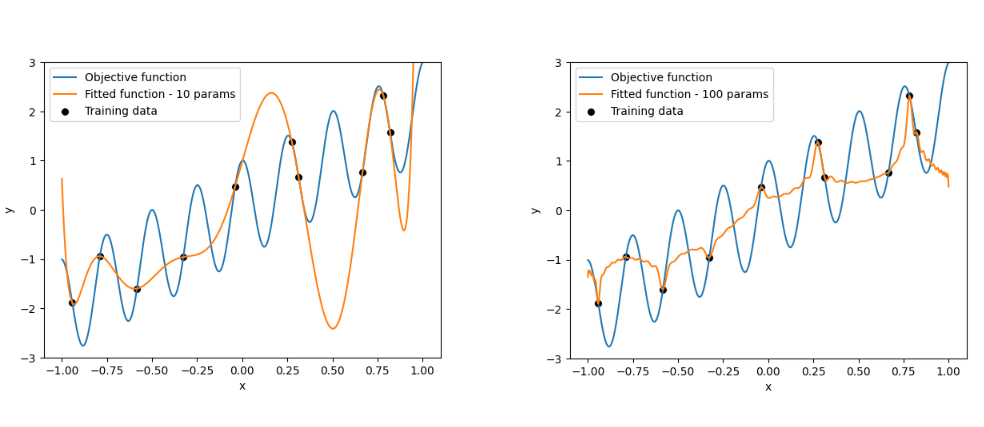
\includegraphics[width=0.8\linewidth]{img/suavidad1.png}
    \caption[Distintos modelos polinómicos para aproximar una función.]{Distintos modelos polinómicos (línea naranja) para aproximar una función objetivo (línea azul). Ambos modelos se ajustan de manera perfecta a los datos de entrenamiento (puntos azules); sin embargo, el segundo modelo generaliza mejor al estar regularizado hacia una solución de norma pequeña. Imagen del autor inspirada en~\cite{Schaeffer2023}.}\label{fig:suavidad1}
\end{figure}

Extrayendo conclusiones de la Figura~\ref{fig:suavidad1} y apoyándonos en la intuición ampliamente compartida dentro de la comunidad científica, se puede postular que una noción adecuada de \textbf{suavidad funcional} podría desempeñar un papel fundamental en la selección del mejor modelo con miras a la generalización.\newline  

La idea de maximizar la suavidad de una función sujeta a la interpolación de los datos representa una forma de actuar según el principio de la navaja de Ockham~\cite{Blumer1987}. Este principio establece que se debe preferir la explicación más simple que sea consistente con las evidencias. En nuestro caso, podemos utilizar como analogía que los datos de entrenamiento representan las evidencias, mientras que la simplicidad se asocia con la ``suavidad'' de la hipótesis a elegir. De esta manera, el principio de la máxima suavidad se puede formular como: ``Elegir la función más suave, de acuerdo con alguna noción de suavidad funcional, entre todas las que son minimizadoras globales''~\cite{Belkin2021}.\newline

Este comportamiento también se encuentra asociado, en cierta medida, al conjunto de hipótesis $\mathcal{H}$ del modelo. Si consideramos dos conjuntos de hipótesis $\mathcal{H}_1$ y $\mathcal{H}_2$, de manera que $\mathcal{H}_1 \subset \mathcal{H}_2$, y sus correspondientes subconjuntos que contienen las hipótesis que son minimizadoras globales, $S_1 \subset \mathcal{H}_1$ y $S_2 \subset \mathcal{H}_2$, entonces, estos conjuntos estan relacionados por la misma inclusión ($S_1 \subset S_2$).\newline

Por tanto, si $\| \cdot \|_{s}$ es cualquier norma funcional, o más generalmente, cualquier funcional, se verifica que

\[
    \min_{g \in S_2} \| g \|_{s} \leq \min_{g \in S_1} \| g \|_{s}.
\]

Suponiendo que $\| \cdot \|_{s}$ es el sesgo inductivo correcto, que mide esa suavidad (por ejemplo, una norma de Sobolev), entonces esperamos que la hipótesis elegida de $S_2$ sea más suave, debido a que este conjunto contiene un mayor número de hipótesis que el conjunto $S_1$ y, por tanto, este conjunto es más adecuado para resolver el problema, lo que lleva a una mejor generalización de la hipótesis elegida.\newline

El principio enunciado anteriormente también permite explicar la aparición del máximo en el error de generalización cerca del umbral de interpolación, ya que en ese punto el modelo se ve forzado a pasar exactamente por cada uno de los puntos de entrenamiento. Esto conduce a una solución única que depende exclusivamente de los datos de entrenamiento, lo que obliga al modelo a seleccionar dicha solución independientemente de su ``suavidad''.\newline

Ligado a esto, Somepalli et al.~\cite{Somepalli2022} analizaron la reproducibilidad de los resultados obtenidos por las mismas redes neuronales a partir del estudio de sus fronteras de decisión. Para nuestro interés, observaron que cerca del umbral de interpolación, y de forma más notable en presencia de ruido, las regiones de decisión tienden a fragmentarse en áreas más pequeñas, las cuales, por lo general, no son reproducibles entre diferentes ejecuciones. En contraste, fuera de este umbral, las regiones de decisión son menores y bien definidas, siendo en cierta medida más ``suaves'', como puede observarse en la Figura~\ref{fig:ground-truth-reproducibility}.\newline

\begin{figure}[h]
    \centering
    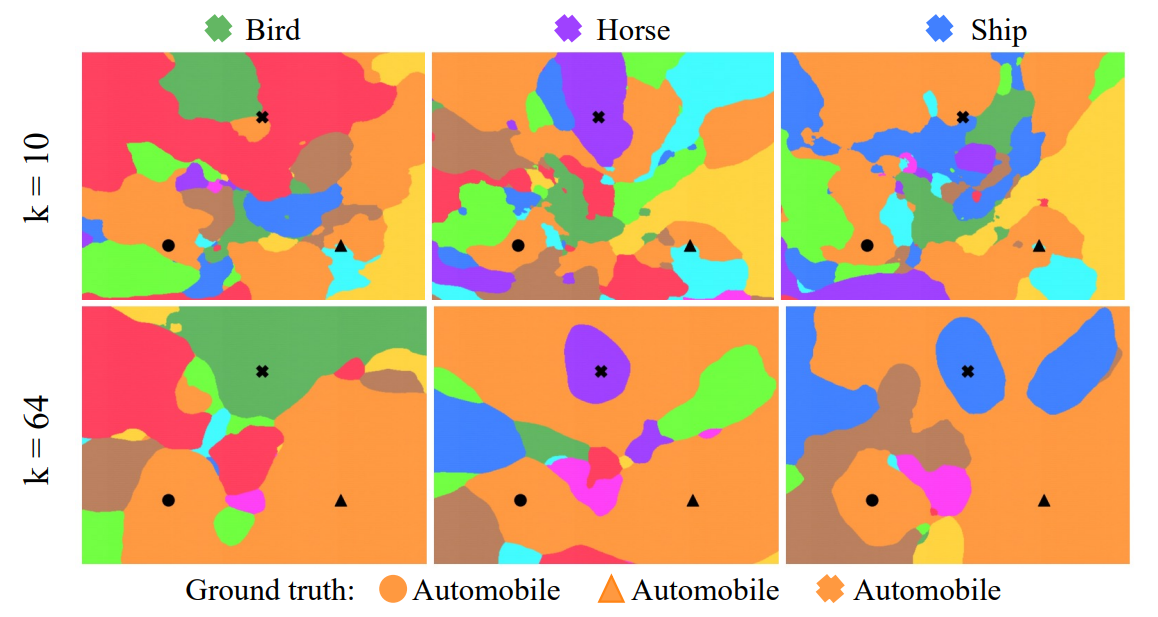
\includegraphics[width=0.6\linewidth]{img/ground-truth-reproducibility.png}
    \caption[Fronteras de decisión para modelos con distinta capacidad~\cite{Somepalli2022}.]{Fronteras de decisión para modelos con distinta capacidad~\cite{Somepalli2022}. Cada columna representa una tripleta distinta de imágenes, en la que una imagen de automóvil (marcada con una $\times$) ha sido etiquetada incorrectamente. El modelo infraparametrizado ($k=10$) genera numerosas regiones de decisión pequeñas y fragmentadas, mientras que el modelo sobreparametrizado ($k=64$) produce un menor número de regiones, más amplias y claramente definidas.}\label{fig:ground-truth-reproducibility}
\end{figure}

Finalmente, a partir de una puntuación de reproducibilidad basada en dichas regiones de decisión, observaron que esta métrica toma valores más bajos cerca del umbral de interpolación. Esto sugiere que, en dicha región, el modelo seleccionado tiende a ser más particular y depende fuertemente de la inicialización de los parámetros de la red utilizada.\newline

Generalmente, puede pensarse que los sesgos inductivos introducidos por los algoritmos de optimización son de naturaleza restrictiva, es decir, imponen restricciones al espacio de hipótesis que están alineadas con el problema de interés. En otras palabras, dado que existen múltiples configuraciones del modelo que se ajustan adecuadamente a los datos pero generan una mala generalización, se prefiere restringir el espacio de hipótesis a aquellas configuraciones que tienden a generalizar mejor para el problema en cuestión, independientemente de si estas son óptimas en un sentido más amplio. Este enfoque está estrechamente relacionado con los principios de regularización.\newline

Además, al reducir el espacio de hipótesis, este se ve más rápidamente limitado por los datos, ya que existen menos opciones para que el modelo se ajuste a ellos. No obstante, estos sesgos restrictivos pueden considerarse, en ciertos contextos, como indeseables. En efecto, lo que se busca es respaldar cualquier solución capaz de describir adecuadamente los datos, lo que implica favorecer un espacio de hipótesis lo suficientemente flexible.\newline

\begin{figure}[h]
    \centering
    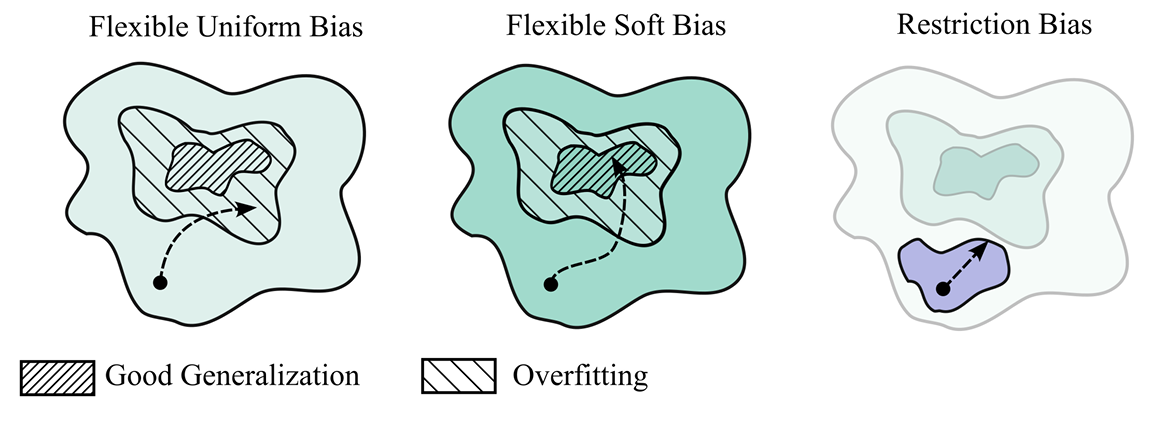
\includegraphics[width=0.6\linewidth]{img/types-of-bias.png}
    \caption[Diferentes tipos de sesgo para el espacio de hipótesis~\cite{Wilson2025}.]{Diferentes tipos de sesgo para el espacio de hipótesis~\cite{Wilson2025}. A la izquierda observamos un conjunto de hipótesis grande sobre el cual no se tiene preferencia por las soluciones que ajustan igualmente bien los datos. En este caso, el entrenamiento puede derivar en soluciones de sobreajuste que generalizan mal. En el centro, se presenta un conjunto de hipótesis flexible en combinación con un sesgo inductivo suave, que guía el entrenamiento hacia soluciones que generalizan bien. A la derecha, restringir el espacio de hipótesis puede ayudar a evitar el sobreajuste al considerar solo algunas soluciones. Sin embargo, al limitar la expresividad del modelo, se impide captar todos los matices de la realidad, lo que dificulta la mejor generalización posible.}\label{fig:types-of-bias}
\end{figure}

La idea general de preferir ciertas soluciones sobre otras, incluso cuando ambas se ajustan igualmente a los datos, se conoce como sesgo inductivo suave~\cite{Wilson2025}. La Figura~\ref{fig:types-of-bias} ilustra este concepto, distinguiéndolo de otros tipos de sesgo.El hecho de considerar estos sesgos inductivos suaves se relaciona directamente con la disminución de la varianza (y, por lo tanto, también del error) a medida que aumentamos la capacidad del modelo. Este tipo de sesgos se centra en una zona específica (y favorable) del espacio de hipótesis, reduciendo así la varianza asociada. Es comparable a utilizar un sesgo restrictivo, pero enfocado en un subconjunto adecuado de hipótesis, como puede observarse en la Figura~\ref{fig:types-of-bias}.\newline

Por otro lado, a medida que aumenta la cantidad de parámetros, también crece el volumen de soluciones planas en el paisaje de la función de pérdida (como se ha observado en la subsección anterior), lo que facilita el acceso y la selección de una de ellas~\cite{Huang2020}. Así, los modelos más grandes (sobreparametrizados) presentan sesgos inductivos más pronunciados, como se puede observar en la Figura~\ref{fig:overparametrization}.\newline

\begin{figure}[h]
    \centering
    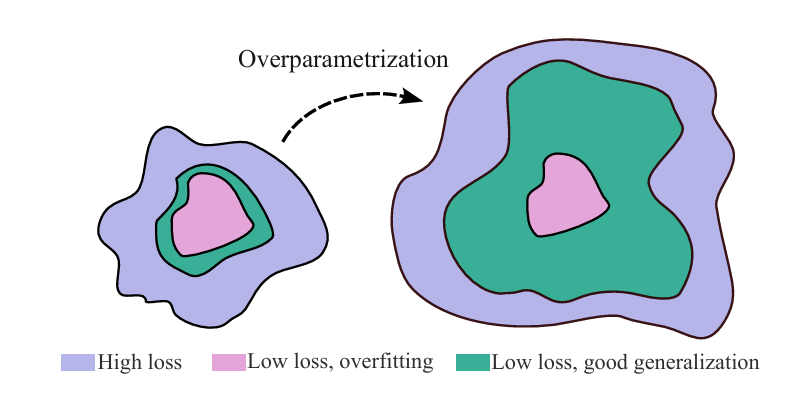
\includegraphics[width=0.5\linewidth]{img/overparametrization.png}
    \caption[Aumentar la capacidad de un modelo mejora su generalización~\cite{Wilson2025}.]{Aumentar la capacidad de un modelo mejora su generalización~\cite{Wilson2025}. Al aumentar el número de parámetros de un modelo, las soluciones ``planas'' ocupan un mayor volumen dentro del espacio total de hipótesis, lo que implica un sesgo inductivo suave hacia estas soluciones simples. Aunque los modelos sobreparametrizados presentan muchas hipótesis que sobreajustan los datos, también pueden contener muchas otras que se ajustan bien a los datos y proporcionan una buena generalización. De este modo, la sobreparametrización puede aumentar simultáneamente el tamaño del espacio de hipótesis y del sesgo hacia soluciones más simples.}\label{fig:overparametrization}
\end{figure}

Ligado a la explicación del fenómeno de la generalización, también surge el siguiente resultado~\cite{Maddox2020}, ampliamente relacionado con lo presentado en la Subsección~\ref{subsec:analisis-intuitivo-minimos-cuadrados}.

\begin{definicion}(Dimensionalidad efectiva)
    Sea $A \in \mathcal{M}_{n \times n}(\mathbb{R})$ una matriz simétrica. Se define su dimensionalidad efectiva como

    \[
        N_{eff}(A) = \sum_{i=1}^{n}\frac{\lambda_i}{\lambda_i + \alpha},
    \]

    donde $\lambda_i$ son los valores propios de la matriz $A$ y $\alpha > 0$ es una constante de regularización.
\end{definicion}

Así, la dimensionalidad efectiva mide el número de valores propios relativamente grandes, lo que puede interpretarse como una medida de las direcciones significativas en el espacio de parámetros. En particular, la dimensionalidad efectiva de la matriz Hessiana de la función de pérdida, evaluada en el vector de parámetros $w$, cuantifica el número de direcciones agudas (direcciones con curvatura) en el paisaje de pérdidas, es decir, el número de parámetros que están determinados por los datos.\newline

Maddox et al.~\cite{Maddox2020} descubrieron que, después del entrenamiento, los modelos grandes tienen menos parámetros efectivos que los modelos más pequeños, al observar su dimensionalidad efectiva. En trabajos más recientes, Goldblum et al.~(2024)~\cite{Goldblum2024} también demostraron que los LLM presentan un fuerte sesgo hacia soluciones más simples, y que este sesgo es una característica clave para un buen rendimiento. Estos resultados refuerzan la conjetura de que las soluciones más simples tienden a obtener mejores resultados, ya que son más comprensibles y siguen la filosofía de Ockham. Asimismo, el sesgo inductivo hacia estas soluciones contrarresta, de alguna manera, el crecimiento del número de soluciones que no son minimizadoras globales~\cite{Mingard2023}.\newline

Como conlusión, podemos decir que el uso de sistemas sobreparametrizados resulta ventajoso para obtener cada vez más soluciones posibles (minimizadores globales) para nuestro problema. De esta forma, al aumentar la capacidad del modelo (en nuestro caso, su complejidad efectiva), resultará más sencillo para el algoritmo de optimización elegir una ``buena'' hipótesis (que generalice mejor que el resto) basada en algún sesgo inductivo que utilice. Este sesgo parece ir ligado hacia soluciones más simples, donde, en el caso de las hipótesis, se pueden entender como más ``suaves'', lo que conduce a la hipótesis elegida a una especie de autoregulación.\newline

\section{Aproximación no lineal}\label{sec:aproximacion-no-lineal}

En esta sección, introduciremos algunos elementos fundamentales de la teoría de la aproximación no lineal~\cite{DeVore1998}, la cual está relacionada con el problema del aprendizaje profundo. Además, desarrollaremos ciertos conceptos con el propósito de demostrar la existencia de analogías entre esta teoría y el fenómeno conocido como \textit{Deep Double Descent}, así como de proporcionar una posible explicación desde esta perspectiva.\newline

Comenzamos recordando que el problema principal de la teoría de la aproximación es encontrar una representación para una función, generalmente compleja, denominada función objetivo $f$, utilizando funciones más simples llamadas \textbf{aproximantes}. De esta manera, al igual que en el caso del aprendizaje, ambos enfoques buscan aproximar una determinada función a partir de otras más sencillas.\newline

La aproximación no lineal implica que los aproximantes no provienen de espacios lineales, sino de variedades no lineales. Dado que el incremento en la resolución de la función objetivo solo puede lograrse aumentando la complejidad de los aproximantes, resulta lógico considerar que la aproximación no lineal ofrece ventajas sobre los métodos clásicos. Para evaluar esto, estudiaremos la tasa de aproximación, definida como la disminución del error en función del número de parámetros en el aproximante, en relación con el doble descenso.\newline

Por tanto, la idea de no restringir las aproximaciones a espacios lineales consiste en utilizar una malla más fina en las regiones donde la función objetivo no es muy suave (presenta singularidades) y una malla más gruesa donde sí lo es. No obstante, será necesario caracterizar formalmente esta noción de suavidad para obtener resultados concluyentes.\newline

Finalmente, nos centraremos en la aproximación no lineal conocida como aproximación de $n$ términos, que consiste en mantener el control únicamente sobre el número de términos a utilizar para realizar la aproximación, dejando que la selección de los términos dependa de la función objetivo. Esto conduce a un problema de doble etapa, en el que la función objetivo se utiliza tanto para seleccionar una base adecuada de una biblioteca de bases como para elegir la mejor aproximación de $n$ términos en relación con dicha base.

\subsection{Aproximación en un espacio de Hilbert}

Dado que los problemas de la teoría de la aproximación son más sencillos de analizar en un espacio de Hilbert, comenzaremos con una breve discusión sobre este entorno, con el fin de introducir los conceptos clave.\newline

Por ello, sea $\mathcal{H}$ un espacio de Hilbert con producto interno $\langle \cdot, \cdot \rangle$ y norma $\|\cdot\|_{\mathcal{H}}$, y sea $\{\eta_k\}_{k=1}^{n}$ una base ortonormal de $\mathcal{H}$. Para el caso de la aproximación lineal, consideramos el espacio lineal $\mathcal{H}_n = \text{span}\{\eta_k : 1 \leq k \leq n\}$ para aproximar un elemento $f \in \mathcal{H}$. El error de aproximación se mide mediante
\[
    E_n(f)_{\mathcal{H}} = \inf_{g \in \mathcal{H}_n} \| f - g \|_{\mathcal{H}}.
\]

Como contraparte en la aproximación no lineal, que es el caso de estudio de este análisis, contamos con la aproximación de $n$ términos, que reemplaza $\mathcal{H}_n$ por el espacio $\Sigma_n$, el cual consiste en todos los elementos $g \in \mathcal{H}$ que pueden expresarse como
\[
    g = \sum_{k \in \Lambda} c_k \eta_k,
\]
donde $\Lambda \subset \mathbb{N}$ es un conjunto de índices con $\# \Lambda \leq n$ (cardinalidad finita).\newline

Se puede verificar que, a diferencia de $\mathcal{H}_n$, el espacio $\Sigma_n$ no es lineal. De manera análoga al error de aproximación lineal $E_n$, definimos el error de aproximación de $n$ términos como

\[
    \sigma_n(f)_{\mathcal{H}} = \inf_{g \in \Sigma_n} \| f - g \|_{\mathcal{H}}.
\]

\begin{definicion}
    Dado un número real $\alpha > 0$, denotamos por $\mathcal{A}^{\alpha}(\Sigma_n)$ la clase de funciones $f \in \mathcal{H}$ que cumplen la siguiente desigualdad para algún $M > 0$:

    \begin{equation}\label{eq:clases-error}
        \sigma_n(f)_{\mathcal{H}} \leq M n^{-\alpha}, \quad n \in \mathbb{N}.
    \end{equation}

    Además, definimos la seminorma $|f|_{\mathcal{A}^{\alpha}(\Sigma_n)}$ como el ínfimo de todos los valores de $M$ para los cuales se cumple la ecuación anterior.
\end{definicion}

Denominaremos al conjunto $\mathcal{A}^{\alpha}$ como un \textbf{espacio de aproximación}, el cual agrupa las funciones $f \in \mathcal{H}$ con un comportamiento de aproximación similar, es decir, aquellas cuyo error de aproximación disminuye con una tasa de orden $n^{-\alpha}$.\newline

Finalmente, podemos caracterizar el espacio $\mathcal{A}^{\alpha}(\Sigma_n)$ reorganizando los coeficientes de la función $f$ de manera decreciente. Denotamos por $\gamma_k(f)$ al $k$-ésimo valor más grande de los coeficientes absolutos de la función $f$. 

\begin{teorema}
    Una función $f \in \mathcal{A}^{\alpha}(\Sigma_n)$ si y solo si se cumple la siguiente desigualdad:

    \begin{equation}\label{eq:coeficientes-reordenados1}
        \gamma_n(f) \leq M n^{-\alpha - 1/2},
    \end{equation}

    donde el ínfimo de todos los $M$ que satisfacen la ecuación anterior es equivalente a la seminorma $|f|_{\mathcal{A}^{\alpha}(\Sigma_n)}$.
\end{teorema}

\begin{proof}
    En primer lugar, notemos que

    \[
        \sigma_n(f)^2_{\mathcal{H}} = \sum_{k>n} \gamma_k(f)^2,
    \]

    dado que el error de aproximación al cuadrado es la suma de los cuadrados de los coeficientes que no están involucrados en la aproximación.\newline

    Por tanto, si $f$ cumple la ecuación~\eqref{eq:coeficientes-reordenados1}, es inmediato que
    \[
        \sigma_n(f)_{\mathcal{H}} \leq C M n^{-\alpha},
    \]

    lo que demuestra que $f \in \mathcal{A}^{\alpha}(\Sigma_n)$. Por otro lado, si $f \in \mathcal{A}^{\alpha}(\Sigma_n)$, entonces se satisface la siguiente desigualdad:

    \[
        \gamma_{2n}(f)^2 \leq n^{-1} \sum_{m=n+1}^{2n} \gamma_m(f)^2 \leq n^{-1} \sigma_n(f)_{\mathcal{H}}^2 \leq |f|_{\mathcal{A}^{\alpha}(\Sigma_n)}^2 n^{-2\alpha - 1} \leq M^2 n^{-2\alpha - 1}.
    \]

    Dado que una desigualdad análoga se verfiica para $\gamma_{2n+1}(f)$, debido a la naturaleza decreciente de los coeficientes $\gamma_k(f)$, se obtiene la implicación restante.\newline
\end{proof}

A su vez, definimos el espacio de aproximación $\mathcal{A}_{\infty}^{\alpha}(\Sigma_n)$ como el conjunto de todas las funciones $f \in \mathcal{H}$ tales que

\[
    \sup_{n \geq 1} n^{\alpha} \sigma_n(f)_{\mathcal{H}} < \infty.
\]

Es decir, este conjunto está compuesto por todas las funciones $f \in \mathcal{H}$ que cumplen que

\[
    \sigma_n(f)_{\mathcal{H}} = O(n^{-\alpha}), \quad n \to \infty.
\]

Esto significa que, para las funciones $f$ en $\mathcal{A}_{\infty}^{\alpha}(\Sigma_n)$, la secuencia de los errores de aproximación $\sigma_n(f)_{\mathcal{H}}$ decrece de manera suficientemente rápida conforme $n$ crece.\newline

Al mismo tiempo, denotamos por $\ell_{p,q}$ los espacios de sucesiones de Lorentz\footnote{Los espacios de Lorentz son generalizaciones de los espacios $L^{p}$, en el sentido de que $\ell_{p}^{p} = L^{p}$, y permiten una caracterización más precisa del comportamiento asintótico de las sucesiones. En particular, los espacios $\ell_{p,\infty}$ corresponden a la versión débil de los espacios $L^{p}$.}. Para nuestro desarrollo, nos centraremos únicamente en el espacio $\ell_{p,\infty}$ (el espacio débil $\ell_{p}$), que está formado por todas las sucesiones que satisfacen

\[
    x^{*}(n) \leq M n^{-1/p},
\]

donde $x^{*}(n)$ es el reordenamiento decreciente de la sucesión $|x(n)|$.\newline

Finalmente, el siguiente resultado nos ayuda a relacionar el espacio de aproximación $\mathcal{A}_{\infty}^{\alpha}$ con el espacio débil $\ell_p$ ($\ell_{p,\infty}$).

\begin{teorema}\label{teo:espaciosapprox-espacioslorentz}
    Para una aproximación de $n$ términos en un espacio de Hilbert $\mathcal{H}$, una función $f \in \mathcal{A}_{\infty}^{\alpha}$ si y solo si sus coeficientes $\{ f_k : k \in \{1, \ldots, n\}\}$ están en el espacio débil $\ell_{\tau}$ (es decir, en $\ell_{\tau, \infty}$) con $\tau = (\alpha + 1/2)^{-1}$. Además, en este caso, se verifica

    \[
        C_1 |f|_{\mathcal{A}_{\infty}^{\alpha}(\mathcal{H})} \leq \| (f_k) \|_{\ell_{\tau, \infty}} \leq C_2 |f|_{\mathcal{A}_{\infty}^{\alpha}(\mathcal{H})},
    \]

    donde $C_1, C_2 > 0$ son constantes.\newline
\end{teorema}

\subsection{Aproximación altamente no lineal}

Nos preguntamos ahora cómo depende la efectividad de la aproximación de $n$ términos de la base elegida y si se puede conseguir alguna ventaja eligiendo de manera progresiva una base que dependa de la función objetivo. Para ello, llamamos \textbf{biblioteca} a una clase $\mathcal{L}$ de bases. Por simplicidad, centraremos nuestra discusión en aproximaciones en un espacio de Hilbert $\mathcal{H}$ y en bibliotecas de bases ortonormales para $\mathcal{H}$.\newline

Por consiguiente, nuestro problema de aproximación cosiste, dada una función objetivo $f \in \mathcal{H}$, en elegir una base $B \in \mathcal{L}$ y una aproximación de $n$ términos a $f$ usando esta base. Llamamos a este tipo de problema de aproximación altamente no lineal, ya que implica una capa adicional de no linealidad en la selección de bases.\newline

No obstante, otra forma de aproximación estrechamente relacionada es la aproximación utilizando $n$ términos desde un \textbf{diccionario} $\mathbb{D} \subset \mathcal{H}$ de funciones, que será nuestro principal objeto de estudio. En nuestro caso, un diccionario se define como un subconjunto arbitrario de $\mathcal{H}$.\newline

Por ejemplo, en el caso de redes neuronales, un diccionario de funciones podría tener la siguiente forma:

\[
    \{ \sigma(w \cdot x + b) : w \in \mathbb{R}^{P}, b \in \mathbb{R} \}
\]

donde $\sigma$ es una función de activación de una variable fija, $w$ es el vector de parámetros y $b$ es el término de sesgo. De esta manera, se aproximan funciones de $P$ variables mediante combinaciones lineales de funciones de dicho conjunto. Generalmente, se requiere que $\sigma$ cumpla con algunas propiedades adicionales (véase Subsección~\ref{subsubsec:capa-de-activacion}).\newline

Otro ejemplo particular de diccionario es utilizar una base ortonormal $B$ para $\mathcal{H}$ y definir el diccionario asociado como sigue:

\[
    \mathbb{D} = \{\pm b : b \in B\},
\]

donde diremos que $\mathbb{D}$ es el diccionario generado por la base $B$.\newline

La característica común de todos los diccionarios es que la familia de funciones utilizada para el proceso de aproximación es \textbf{redundante}. Es decir, hay muchas más funciones en el diccionario de las necesarias para aproximar cualquier función objetivo $f \in \mathcal{H}$. Por tanto, buscamos que esta redundancia incremente la eficiencia de la aproximación, aunque, por otro lado, también podría ralentizar el proceso de búsqueda de buenas aproximaciones.\newline

\subsubsection{Selección óptima de bases}\label{subsubsec:seleccion-optima-bases}

En esta subsección trataremos cómo la selección adecuada de una base influye directamente en el error de aproximación. Asimismo, observaremos que, al disponer de una biblioteca de bases, el error de aproximación se minimiza para cualquier aproximación realizada, ya que se consideran todas las bases disponibles.\newline

Sea $B = \{ \eta_k \}$ una base ortonormal para $\mathcal{H}$ y sea $\Sigma_n(B)$ el conjunto de funciones en $\mathcal{H}$ que pueden escribirse como una combinación lineal de $n$ de las funciones $\eta_k$, con $k \in \mathbb{N}_0$. Además, definimos

\[
    \sigma_n(f, B) = \sigma_n(f,B)_{\mathcal{H}} = \inf_{S \in \Sigma_n(B)} \| f - S \|_{\mathcal{H}}
\]

como el error de aproximación correspondiente respecto a la base $B$.\newline

Recordemos que la disminución de los errores de aproximación $\sigma_n(f, B)$ está completamente determinada por los coeficientes reorganizados de la función $f$. Como antes, sea $\gamma_k(f, B)$ el $k$-ésimo mayor valor absoluto de estos coeficientes. Aplicando el Teorema~\ref{teo:espaciosapprox-espacioslorentz} a los coeficientes $\gamma_n(f, B)$, sabemos que $f \in \mathcal{H}$ está en $\mathcal{A}_\infty^\alpha (\mathcal{H}, B)$, si y solo si $(\gamma_n(f, B))$ está en $\ell_{\tau}$ con $\tau = (\alpha + 1/2)^{-1}$. Además, 

\begin{equation}\label{eq:bases}
    C_1 |f|_{\mathcal{A}_\infty^\alpha} \leq \| \gamma_n(f, B) \|_{\ell_{\tau, \infty}} \leq C_2 |f|_{\mathcal{A}_\infty^\alpha},
\end{equation}

con constantes de equivalencia independientes de la base $B$ elegida.\newline

Supongamos ahora que $\mathcal{L} = \{ B_1, \ldots, B_n \}$ es una biblioteca de bases ortonormales. Definimos el error de aproximación con respecto a $\mathcal{L}$ como sigue

\[
    \sigma_n^{\mathcal{L}}(f)_{\mathcal{H}} = \inf_{B \in \mathcal{L}} \sigma_n(f, B)_{\mathcal{H}}.
\]

A la vista de la Ecuación~\eqref{eq:bases}, obtenemos la siguiente cota superior

\begin{equation}\label{eq:bases2}
    \sigma_n^{\mathcal{L}}(f)_{\mathcal{H}} \leq C n^{-\alpha} \inf_{B} \| \gamma_n(f, B) \|_{\ell_r, \infty}
\end{equation}

con $C$ una constante absoluta. Además, para cualquier $\alpha > 0$, se tiene

\begin{equation}\label{eq:bases3}
    \bigcap_{B} \mathcal{A}_\infty^\alpha (\mathcal{H}, B) \subset \mathcal{A}_\infty^\alpha (\mathcal{H}, \mathcal{L}).
\end{equation}

En consecuencia, para cada base ortonormal $B$, la condición $(\gamma_n(f)) \in \ell_{\tau, \infty}$, $\tau = (\alpha + 1/2)^{-1}$, puede verse como una condición de suavidad de la función $f$ relativa a la base $B$. Así, el ínfimo en el lado derecho de la Ecuación~\eqref{eq:bases2} puede interpretarse como el ínfimo de condiciones de suavidad relativas a las diferentes bases $B$.\newline

De manera similar, podemos ver las clases $\mathcal{A}_\infty^\alpha (\mathcal{H}, B)$ como clases de suavidad con respecto a la base $B$. De esta forma, una ventaja de la selección óptima de bases es que siempre podemos elegir la base $B \in \mathcal{L}$ en la que $f$ sea más suave.\newline

Por su parte, las Ecuaciones~\eqref{eq:bases2} y~\eqref{eq:bases3} muestran que la base más eficiente para aproximar $f$ depende del número de términos utilizados para la aproximación. De esta forma, se pueden construir dos bases, $B_1$ y $B_2$, y una función objetivo $f$ de tal manera que, para ciertos valores de $n$, la elección óptima de base varíe entre $B_1$ y $B_2$. Es decir, para algunos valores de $n$, $B_1$ ofrecerá un mejor error de aproximación, mientras que para otros, $B_2$ es más eficiente, lo que demuestra que no hay una base universalmente mejor para todos los valores de $n$.\newline

\subsubsection{Aproximación usando $n$ términos de un diccionario}\label{subsubsec:approx-n-terms}

Supongamos que $\mathbb{D}$ es un diccionario de funciones en $\mathcal{H}$. Para simplificar, asumimos (sin pérdida de generalidad en la aproximación de $n$ términos) que cada $g \in \mathbb{D}$ tiene norma uno, es decir, $\|g\|_{\mathcal{H}} = 1$, y que $-g \in \mathbb{D}$ siempre que $g \in \mathbb{D}$.\newline

Para cada $n \in \mathbb{N}$, definimos $\Sigma_n := \Sigma_n(\mathbb{D})$ como la colección de todas las funciones en $\mathcal{H}$ que pueden expresarse como una combinación lineal de, como máximo, $n$ elementos de $\mathbb{D}$. Así, cada función $S \in \Sigma_n$ puede escribirse de la forma:

\begin{equation}\label{eq:n-terms1}
    S = \sum_{g \in \Lambda} c_g g, \quad \Lambda \subset \mathbb{D}, \quad \#\Lambda \leq n,
\end{equation}

donde $c_g \in \mathbb{R}$ son los coeficientes y $\#\Lambda$ denota el cardinal del conjunto $\Lambda$. Cabe destacar que un elemento de $\Sigma_n(\mathbb{D})$ puede expresarse de la forma~\eqref{eq:n-terms1} de más de una forma.\newline

\begin{definicion}
    Para una función $f \in \mathcal{H}$, definimos su error de aproximación a partir de un diccionario $\mathbb{D}$ como:

    \[
        \sigma_n(f) := \sigma_n(f, \mathbb{D})_{\mathcal{H}} := \inf_{S \in \Sigma_n} \| f - S \|_{\mathcal{H}}.
    \]
\end{definicion}

Así, nuestro interés se centra en obtener estimaciones para $\sigma_n$ (tanto superiores como inferiores). Para este propósito, introducimos la siguiente forma de medir la suavidad con respecto a un diccionario $\mathbb{D}$.\newline

\begin{definicion}
    Para un diccionario $\mathbb{D}$ y cualquier $\tau > 0$, definimos la clase de funciones:

    \[
        \mathcal{K}_{\tau}^{o}(\mathbb{D}, M) := \left\{ f = \sum_{g \in \Lambda} c_g g : \Lambda \subset \mathbb{D}, \quad \#\Lambda < \infty \quad \text{y} \quad \sum_{g \in \Lambda} |c_g|^{\tau} \leq M^{\tau} \right\},
    \]

    y definimos $\mathcal{K}_{\tau}(\mathbb{D}, M)$ como la clausura en $\mathcal{H}$ de $\mathcal{K}_{\tau}^{o}(\mathbb{D}, M)$. Además, definimos $\mathcal{K}_{\tau}(\mathbb{D})$ como la unión de las clases $\mathcal{K}_{\tau}(\mathbb{D}, M)$ para todo $M > 0$. Para $f \in \mathcal{K}_{\tau}(\mathbb{D})$, definimos la seminorma:

    \[
        |f|_{\mathcal{K}_{\tau}(\mathbb{D})} = \inf\{ M : f \in \mathcal{K}_{\tau}(\mathbb{D}, M) \}.
    \]
\end{definicion}

En otras palabras, $\mathcal{K}_{\tau}^{o}(\mathbb{D}, M)$ está formado por la clase de funciones que se pueden escribir como una combinación lineal de un número finito de elementos de $\mathbb{D}$, de tal manera que la suma de los coeficientes elevados a la potencia $\tau$ se encuentre acotada, controlando así la magnitud de las combinaciones lineales.\newline

Por otro lado, $|f|_{\mathcal{K}_{\tau}(\mathbb{D})}$ nos indica la dificultad de aproximar una función $f$ utilizando una combinación de funciones del diccionario. Cuanto más pequeña sea la seminorma, más sencillo será aproximar la función $f$.\newline

\begin{observacion}
    Cuando $\tau = 1$, $\mathcal{K}_1$ es la clase de funciones que son una combinación convexa de las funciones en $\mathbb{D}$.\newline
\end{observacion}

Para el caso en el que $\mathbb{D}$ es generado por una base $B$ se sigue que la aproximación de $n$ términos desde $\mathbb{D}$ es la misma que la aproximación de $n$ términos desde $B$. En particular, si $\tau = (\alpha + 1/2)^{-1}$ y $B$ es ortonormal, se verifica que:

\begin{equation}\label{eq:n-terms-error}
    \sigma_n(f, \mathbb{D})_{\mathcal{H}} \leq Cn^{-\alpha} |f|_{\mathcal{K}_{\tau}(\mathbb{D})}.
\end{equation}

Sabemos que $Cn^{-\alpha}$ es un factor de decaimiento que describe cómo el error de aproximación disminuye a medida que incrementamos el número de términos $n$ en la aproximación. La constante $C$ es un valor positivo que depende tanto del diccionario como de la función, mientras que la potencia $\alpha$ depende de $\tau$ y de las propiedades de la función objetivo.\newline

De esta forma, la Ecuación~\eqref{eq:n-terms-error} nos proporciona una cota superior para el error de aproximación de una función $f$ utilizando una aproximación de $n$ términos, a partir de un diccionario $\mathbb{D}$ generado por una base ortonormal $B$. En consecuencia, el error de aproximación $\sigma_n(f, \mathbb{D})_{\mathcal{H}}$ depende tanto de la suavidad de la función $f$ (medida por $|f|_{\mathcal{K}_{\tau}(\mathbb{D})}$) como del número de términos $n$ empleados en la aproximación.\newline

Finalmente, estamos interesados en verificar si la Ecuación~\eqref{eq:n-terms-error} es válida para diccionarios más generales. El siguiente resultado nos proporciona una cota superior para el error de aproximación en estos casos, extendiendo los resultados obtenidos en el caso de diccionarios generados por bases ortonormales.

\begin{teorema}
    Sean $\mathbb{D}$ un diccionario de funciones, $\alpha \geq 1/2$ y $1/\tau = \alpha + 1/2$. Si $f \in K_{\tau}(\mathbb{D})$, entonces

    \begin{equation}\label{eq:n-terms-teo}
        \sigma_m(f, \mathbb{D})_{\mathcal{H}} \leq C |f|_{K_{\tau}(\mathbb{D})} m^{-\alpha} \quad \forall m \in \mathbb{N},
    \end{equation}

    donde $C$ depende de $\tau$.
\end{teorema}

\begin{proof}
    Es suficiente probar la desigualdad~\eqref{eq:n-terms-teo} para funciones $f$ que puedan expresarse como una suma finita $f = \sum_j c_j g_j$, con $g_j \in \mathbb{D}$ y $\sum_j |c_j|^\tau \leq M^\tau$. Sin pérdida de generalidad, podemos suponer que los coeficientes $c_j$ son positivos y están ordenados de manera decreciente.\newline
    
    Definimos la suma parcial de los primeros $n$ términos como $s_1 = \sum_{j=1}^{n} c_j g_j$ y su residuo asociado como $R_1 = f - s_1 = \sum_{j>n} c_j g_j$. Ahora,

    \[
        c_n^\tau \leq \frac{1}{n} \sum_{j=1}^{n} |c_j|^\tau \leq \frac{M^\tau}{n}, \quad n \in \mathbb{N}.
    \]

    Por tanto, tomando la raíz $ \tau $-ésima de ambos lados, y dado que los coeficientes están ordenados de manera decreciente, tenemos que $ c_j \leq M \cdot n^{-1/\tau} $ para $ j > n $, lo que nos lleva a

    \[
        \sum_{j>n} c_j = \sum_{j>n} c_j^{1-\tau} c_j^\tau \leq M^{1-\tau} n^{1-1/\tau} \sum_{j>n} c_j^\tau \leq M n^{1-1/\tau}.
    \]

    Esto implica que $R_1$ pertenece a $K_1(\mathbb{D}, M n^{1 - 1/\tau})$. Haciendo uso del Teorema 3.2 de~\cite{DeVore1996}, existe una función $s_2$ que es una combinación lineal de a lo sumo $n$ de los elementos $g \in \mathbb{D}$ tal que

    \[
        \| f - (s_1 + s_2) \| = \| R_1 - s_2 \| \leq 2M n^{1-1/\tau} n^{-1/2} = 2M n^{-\alpha},
    \]

    de donde se obtiene la desigualdad~\eqref{eq:n-terms-teo}.\newline
\end{proof}

\subsection{Analogía con el \textit{Deep Double Descent}}\label{subsec:analogia-matematica-ddd}

A modo de conclusión de este inciso sobre la teoría de la aproximación no lineal, presentaremos a lo largo de esta sección las similitudes que existen entre dicha teoría y el doble descenso, con el objetivo de establecer ciertas analogías que ofrezcan ideas matemáticas subyacentes asociadas a su ocurrencia.\newline

En primer lugar, el objetivo tanto de la aproximación no lineal como del aprendizaje es esencialmente el mismo: aproximar una función objetivo mediante funciones más simples. En el contexto de la teoría de la aproximación, se suele asumir que se conocen los valores de ciertos funcionales lineales simples aplicados a la función objetivo. En cambio, en el aprendizaje, dicha función es completamente desconocida y solo se tiene acceso a un conjunto finito de observaciones. Asimismo, en ambos contextos se recurre al uso de funciones no lineales para aproximar la función objetivo, lo que permite capturar comportamientos complejos que no podrían representarse adecuadamente mediante aproximaciones provenientes de espacios lineales.\newline

La base a partir de la cual se construyen los aproximantes también desempeña un papel fundamental. Aunque en el caso de las redes neuronales lo que se utiliza propiamente es un diccionario, este diccionario será dependiente de la base elegida. De esta manera, cuando llevemos a cabo los experimentos relacionados con la aproximación polinómica mediante el uso de la pseudoinversa, veremos cómo la elección de la base influye de manera significativa en los resultados obtenidos. En consecuencia, observaremos cómo el error de aproximación obtenido depende efectivamente de la base elegida, tal como se discutió en la Subsección~\ref{subsubsec:seleccion-optima-bases}, y corroboraremos que ciertas bases resultan más adecuadas para aproximar determinadas funciones. De este modo, se puede intuir que los modelos de aprendizaje obtienen sus aproximantes a partir de la base elegida hasta alcanzar el umbral de interpolación. Precisamente en ese umbral, el aproximante queda determinado de forma única por el uso completo de la base, lo cual explica que su error de generalización no esté controlado y pueda alcanzar valores elevados.\newline

Por otra parte, al superar el umbral de interpolación, la base pasa a funcionar como un diccionario: un conjunto redundante de funciones en el que, a medida que aumenta el número de parámetros del modelo, se incorporan nuevas posibilidades de aproximación. Aunque estas funciones adicionales son redundantes, contribuyen a mejorar la capacidad de generalización del modelo, ya que al contar con un mayor número de posibles soluciones, el nuevo conjunto de hipótesis resulta más adecuado para resolver el problema. De hecho, como se observó en la Subsección~\ref{subsubsec:approx-n-terms}, la función objetivo tiende a verse más “suave” a medida que aumenta el diccionario. Finalmente, la elección de una ``buena'' hipótesis de todas las disponibles en el diccionario vendría dada por algún sesgo inductivo del algoritmo de optimización utilizado, tal y como se comentó en la Subsección~\ref{subsec:suavidad-funcional}.

\section{Discusión final}\label{sec:conclusion-matematica}

En esta sección hemos expuesto de forma teórica y detallada el \textit{Deep Double Descent}, unificando el enfoque clásico con la práctica moderna a partir de la noción de complejidad efectiva como medida de complejidad del modelo. A partir de esta definición, se identifican las distintas regiones de comportamiento de un modelo durante el entrenamiento, siendo de especial interés la región sobreparametrizada, en la cual hemos centrado nuestro análisis.\newline

Al mismo tiempo, a partir de la descomposición del error en la suma de sesgo y varianza, se introducen las distintas configuraciones que puede adoptar el error de un modelo. Entre ellas, destaca el fenómeno del doble descenso, el cual surge debido a que el sesgo y la varianza predominan en diferentes regiones del comportamiento del modelo, siendo la varianza la que presenta un comportamiento unimodal. También destacamos que, en la región sobreparametrizada, el conjunto de hipótesis disponibles es mayor. De este modo, el verdadero desafío para comprender el fenómeno reside en entender por qué el algoritmo de aprendizaje selecciona ciertas soluciones dentro de ese conjunto sobre otras, y por qué las hipótesis elegidas tienden a generalizar bien.\newline

A partir de un ejemplo de regresión, se introduce un análisis intuitivo del suceso, en el que se observa que su aparición está estrechamente vinculada al término de la varianza. En particular, se verifica que el máximo del error se produce cerca del umbral de interpolación, debido a la configuración de los valores propios que surgen al resolver el problema de regresión.\newline

Posteriormente, se analiza la convergencia del descenso de gradiente, demostrando que, bajo ciertas hipótesis, dicho algoritmo converge hacia soluciones que son minimizadoras globales en la región sobreparametrizada. Esta propiedad se observa tanto en problemas de regresión como en escenarios con datos separables.\newline

A continuación, se presenta la región sobreparametrizada desde el punto de vista de la optimización. En esta sección, se evidencia la existencia de múltiples soluciones dentro de dicha región, así como la ausencia de convexidad local de la función de pérdida en cualquier vecindad de dichas soluciones. Igualmente, se destaca que, mientras en la zona infraparametrizada las soluciones aparecen de forma aislada, en la zona sobreparametrizada estas conforman variedades continuas. Finalmente, se introduce una propiedad más débil que la convexidad, la cual debe cumplir la función de pérdida para garantizar que el descenso de gradiente converja hacia un mínimo global en la región sobreparametrizada. A pesar de conocer la existencia de múltiples soluciones en la región moderna, es necesario entender por qué el algoritmo de aprendizaje tiende a seleccionar aquellas que generalizan adecuadamente. Para ello, se introduce, de forma informal, un concepto de suavidad funcional que orienta al modelo hacia hipótesis más simples, en línea con la filosofía de Ockham. De este modo, el algoritmo de aprendizaje induce un sesgo inductivo suave que lo lleva a concentrarse en subconjuntos óptimos dentro del espacio de hipótesis, lo que contribuye a reducir la varianza en esta región.\newline

Para finalizar esta sección, se introducen conceptos básicos de la teoría de la aproximación no lineal, vinculándolos con el dilema del aprendizaje. A su vez, se presentan ciertas analogías con el doble descenso, mostrando cómo el uso de diccionarios con funciones redundantes permite obtener mejores aproximaciones de la función objetivo. Asimismo, se detallan nociones de suavidad en dichos espacios, reforzando la conexión entre la estructura del modelo y su capacidad de generalización.\newline

Para cerrar este análisis, se presenta la Tabla~\ref{tabla:tabla-conclusion} como resumen de lo que ocurre en las distintas zonas de actuación de un modelo.

\begin{table}[h]
    \centering
    \small 
    \renewcommand{\arraystretch}{0.9} 
    \begin{NiceTabular}{c|c|c|}[color-inside]
        \Block{3-1}{} & \Block[draw, fill={cyan!50}]{3-1}{\textbf{Régimen clásico} \\ \textbf{(infraparametrizado)}} & \Block[draw, fill={cyan!50}]{3-1}{\textbf{Régimen moderno} \\ \textbf{(sobreparametrizado)}} \\ \\ \\

        \hline
        \Block[draw]{3-1}{Conjunto de \\ hipótesis} & \Block[draw]{3-1}{Conjunto subóptimo \\ debido a un sesgo restrictivo} & \Block[draw]{3-1}{Conjunto óptimo \\ debido a un sesgo inductivo suave} \\ \\ \\
        
        \hline
        \Block[draw]{3-1}{Curva de \\ generalización} & \Block[draw]{3-1}{Forma clásica de ``U''} & \Block[draw]{3-1}{Descendiente} \\ \\ \\

        \hline
        \Block[draw]{5-1}{Paisaje de \\ \\ optimización} & \Block[draw]{5-1}{Localmente convexo \\ \\ Mínimos locales aislados} & \Block[draw]{5-1}{No localmente convexo \\ Múltiples mínimos globales formando \\ variedades continuas \\ Cumple la condición $\mu$-PL} \\ \\ \\ \\ \\

        \hline
        \Block[draw]{3-1}{Modelo óptimo} & \Block[draw]{3-1}{\text{Sweet spot} (mínimo de la curva ``U'') \\ (difícil de conseguir)} & \Block[draw]{3-1}{Cualquier minimizador global \\ (fácil de encontrar)} \\ \\ \\

        \hline
        \Block[draw]{3-1}{Convergencia del GD} & \Block[draw]{3-1}{GD converge a un mínimo local} & \Block[draw]{3-1}{GD converge a un mínimo global} \\ \\ \\
        \hline

        \hline
        \Block[draw]{3-1}{Aproximación no lineal} & \Block[draw]{3-1}{Uso de bases (simplicidad/eficiencia) \\ para la aproximación} & \Block[draw]{3-1}{Uso de diccionarios (redundancia) \\ para la aproximación} \\ \\ \\
        \hline


    \end{NiceTabular}
    \caption[Resumen comparativo entre el paradigma clásico y el paradigma moderno.]{Resumen comparativo entre el paradigma clásico y el paradigma moderno.}\label{tabla:tabla-conclusion}
\end{table}

\endinput